%!TEX TS-program = xelatex
%!TEX options = -aux-directory=Debug -shell-escape -file-line-error -interaction=nonstopmode -halt-on-error -synctex=1 "%DOC%"
\documentclass{article}
\input{LaTeX-Submodule/template.tex}

% Additional packages & macros
\usepackage{subcaption}
\usepackage{algorithm}
\usepackage{algpseudocode}
\usepackage{algorithmicx}
\usepackage{nicematrix}

\DeclareMathOperator{\argmin}{arg\, min}

% Header and footer
\newcommand{\unitName}{Computational Mathematics 2}
\newcommand{\unitTime}{Semester 1, 2024}
\newcommand{\unitCoordinator}{Dr Elliot Carr}
\newcommand{\documentAuthors}{Tarang Janawalkar}

\fancyhead[L]{\unitName}
\fancyhead[R]{\leftmark}
\fancyfoot[C]{\thepage}

% Copyright
\usepackage[
    type={CC},
    modifier={by-nc-sa},
    version={4.0},
    imagewidth={5em},
    hyphenation={raggedright}
]{doclicense}

\date{}

\begin{document}
%
\begin{titlepage}
    \vspace*{\fill}
    \begin{center}
        \LARGE{\textbf{\unitName}} \\[0.1in]
        \normalsize{\unitTime} \\[0.2in]
        \normalsize\textit{\unitCoordinator} \\[0.2in]
        \documentAuthors
    \end{center}
    \vspace*{\fill}
    \doclicenseThis
    \thispagestyle{empty}
\end{titlepage}
\newpage
%
\tableofcontents
\newpage
%
\section{Transport Problems}
\subsection{Transport Phenomena}
Transport phenomena broadly comprises three disciplines; fluid
dynamics, heat transfer, and mass transfer.\ \textbf{Fluid dynamics} is
the study of the motion of fluids, including liquids and gases.\
\textbf{Heat transfer} is the study of how heat (thermal energy) is
transported, generated, dissipated, and/or converted in a physical
system.\ \textbf{Mass transfer} is the study of the movement of mass
from one location to another. The mathematical equations used to
describe the above phenomena involve three fundamental mechanisms of
transport:
\begin{enumerate}
    \item \textbf{Diffusion}: The gradual movement of a substance from regions of high
          concentration to regions of low concentration. The direction of
          diffusion is determined by the sign of the negative gradient of the
          concentration.
    \item \textbf{Advection}: The transport of a substance by bulk motion of a fluid.
          Advection is driven by a vector field in which the substance is
          transported.
    \item \textbf{Reaction}: The process in which substances are created or destroyed.
          Reaction is represented as a source or sink function.
\end{enumerate}
\subsection{The Transport Equation}
The general form of the transport equation is given by
\begin{equation*}
    \underbrace{\pdv{u}{t}}_{\text{unsteady term}} + \underbrace{\symbf{\nabla} \cdot \left( \symbf{v} u \right) \vphantom{\pdv{u}{t}}}_{\text{advection term}} = \underbrace{\symbf{\nabla} \cdot \left( \symbf{D} \symbf{\nabla} u \right) \vphantom{\pdv{u}{t}}}_{\text{diffusion term}} + \underbrace{R \vphantom{\pdv{u}{t}}}_{\text{reaction term}}
\end{equation*}
where \(u\left( \symbf{x},\: t \right)\) is the quantity being transported
at position \(\symbf{x}\) and time \(t\), \(\symbf{v}\left( \symbf{x},\: t \right) \in \R^n\)
is a velocity vector field which drives \(u\),
\(\symbf{D} \in \R^{n \times n}\) is the diffusion matrix, and
\(R\left( \symbf{x},\: t \right)\) is a reaction term.\ \(n\) represents
the dimension of the spatial domain of the problem, which can be 1, 2,
or 3.

An alternative form of the transport equation combines the divergence
terms
\begin{equation*}
    \underbrace{\pdv{u}{t} \vphantom{\pdv{u}{t}}}_{\text{unsteady term}} + \underbrace{\symbf{\nabla} \cdot \symbf{q} \vphantom{\pdv{u}{t}}}_{\text{flux term}} = \underbrace{R \vphantom{\pdv{u}{t}}}_{\text{reaction term}}
\end{equation*}
where \(\symbf{q} = \symbf{v} u - \symbf{D} \symbf{\nabla} u\) is the
\textit{flux vector}. This PDE is defined on an open connected subset
\(\Omega \subset \R^n\) with the boundary \(\partial \Omega\).
\subsubsection{Derivation}
The transport equation can be derived from the conservation of mass
principle: the rate of change of the quantity \(u\) within a region
\(D\) must be balanced by the net flow of \(u\) in/out of the boundary
\(\partial{D}\) of \(D\), and the rate of creation or destruction of
\(u\) within \(D\). Consider an arbitrarily small sub-domain \(D\) of
\(\Omega\) with boundary \(\partial D\), then:
\begin{align*}
    \biggl\{ \parbox[c]{2.5cm}{\centering Rate of change                                                                                                          \\ of \(u\) in \(D\)} \biggr\} & =
    -\biggl\{ \parbox[c]{2cm}{\centering \(u\) leaving \(D\)                                                                                                      \\ across \(\partial{D}\)} \biggr\}
    + \biggl\{ \parbox[c]{4cm}{\centering Generation/Destruction                                                                                                  \\of \(u\) within \(D\)} \biggr\} \\
    \odv{}{t} \int_D u \odif{V}                                                    & = -\int_{\partial{D}} \symbf{q} \cdot \symbf{n} \odif{s} + \int_D R \odif{V} \\
    \int_D \pdv{u}{t} \odif{V}                                                     & = -\int_{D} \symbf{\nabla} \cdot \symbf{q} \odif{V} + \int_D R \odif{V}      \\
    \int_D \left( \pdv{u}{t} + \symbf{\nabla} \cdot \symbf{q} - R \right) \odif{V} & = 0                                                                          \\
    \pdv{u}{t} + \symbf{\nabla} \cdot \symbf{q}                                    & = R.
\end{align*}
\subsection{Special Cases}
\subsubsection{One Spatial Dimension}
In one spatial dimension, the transport equation reduces to
\begin{equation*}
    \pdv{u}{t} + \pdv{}{x} \left( v u \right) = \pdv{}{x} \left( D \pdv{u}{x} \right) + R.
\end{equation*}
where \(u\left( x,\: t \right)\) is a function of one spatial dimension
and time, \(v\) is the velocity, and \(D > 0\) is the diffusivity.
\subsubsection{Two Spatial Dimensions}
In two spatial dimensions, the transport equation reduces to
\begin{equation*}
    \pdv{u}{t} + \pdv{}{x} \left( v_x u \right) + \pdv{}{y} \left( v_y u \right) = \pdv{}{x} \left( D_{xx} \pdv{u}{x} \right) + \pdv{}{y} \left( D_{yy} \pdv{u}{y} \right) + R.
\end{equation*}
where \(u\left( x,\: y,\: t \right)\) is a function of two spatial
dimensions and time, \(v_x\) and \(v_y\) are the velocities in the \(x\)
and \(y\) directions, and \(D_{xx}\) and \(D_{yy}\) are the diffusivities
in the \(x\) and \(y\) directions.
\subsubsection{Eliminating Terms}
The transport equation is also called the
\textit{advection-diffusion-reaction equation}.
\begin{itemize}
    \item If the \textit{velocity term} \(\symbf{v}\) is the zero
          vector, the equation reduces to the
          \textit{diffusion-reaction equation}.
    \item If the \textit{diffusion term} \(\symbf{D}\) is the zero
          matrix, the equation reduces to the
          \textit{advection-reaction equation}.
    \item If the \textit{reaction term} \(R\) is zero, the equation
          reduces to the \textit{advection-diffusion equation}.
\end{itemize}
\subsection{Classification}
While the terms in the transport equation may be constant or variable,
certain combinations of these terms lead to different solution methods.
\begin{itemize}
    \item The velocity vector \(\symbf{v}\) may be a constant vector or
          a function of space \(\symbf{x}\), time \(t\), and/or the
          solution \(u\).
    \item The diffusion matrix \(\symbf{D}\) may be a constant matrix
          or a function of space \(\symbf{x}\), time \(t\), and/or the
          solution \(u\).
    \item The reaction term \(R\) may be a constant or a function of
          space \(\symbf{x}\), time \(t\), and/or the solution \(u\).
\end{itemize}
When \(\symbf{v}\) and \(\symbf{D}\) are \underline{not} functions of \(u\), and
\(R\) is a \underline{linear} function of \(u\), the transport equation is
called \textit{linear}. The equation is \textit{nonlinear} otherwise.
The domain \(\Omega\) is called \textit{heterogeneous} if any of the
coefficients \(\symbf{v}\), \(\symbf{D}\), or \(R\) are functions of
space \(\symbf{x}\), and \textit{homogeneous} otherwise.
\subsection{Dimensional Analysis}
Performing a dimensional analysis on the transport equation allows us
to associate physical units with the coefficients of the equation. This
analysis is useful for verifying the correctness of the equation and
for scaling the equation to a dimensionless form. The terms in the
equation
\begin{equation*}
    \pdv{u}{t} + \symbf{\nabla} \cdot \left( \symbf{v} u \right) = \symbf{\nabla} \cdot \left( \symbf{D} \symbf{\nabla} u \right) + R
\end{equation*}
may only be added or subtracted if they have the same units. Therefore,
given that
\begin{equation*}
    \left[ \pdv{u}{t} \right] \equiv \frac{\left[ u \right]}{\left[ t \right]} = \frac{\left[ u \right]}{\mathsf{T}}
\end{equation*}
we can deduce the units of other terms in the equation.
\begin{align*}
    \left[ \symbf{\nabla} \cdot \left( \symbf{v} u \right) \right] \equiv \frac{\left[ \symbf{v} \right] \left[ u \right]}{\left[ x \right]} = \frac{\left[ u \right]}{\mathsf{T}}                                                                                                        & \implies \left[ \symbf{v} \right] = \frac{\mathsf{L}}{\mathsf{T}}   \\
    \left[ \symbf{\nabla} \cdot \left( \symbf{D} \symbf{\nabla} u \right) \right] \equiv \frac{\left[ \symbf{D} \right] \left[ \symbf{\nabla} u \right]}{\left[ x \right]} = \frac{\left[ \symbf{D} \right] \left[ u \right]}{{\left[ x \right]}^2} = \frac{\left[ u \right]}{\mathsf{T}} & \implies \left[ \symbf{D} \right] = \frac{\mathsf{L}^2}{\mathsf{T}} \\
    \left[ R \right] \equiv \frac{\left[ u \right]}{\left[ t \right]}                                                                                                                                                                                                                     & \implies \left[ R \right] = \frac{\left[ u \right]}{\mathsf{T}}
\end{align*}
\subsection{Initial and Boundary Conditions}
In addition to the transport equation, which describes the behaviour of
\(u\) within the domain \(\Omega\), the problem must also specify how
\(u\) behaves at the boundary \(\partial \Omega\) with \textit{boundary
conditions}. Some common boundary conditions include:
\begin{itemize}
    \item Specified value: \(u\left( \symbf{x},\: t \right) = u_b\) on
          \(\partial \Omega\)
    \item Specified flux: \(\symbf{q} \cdot \symbf{n} = q_b\) on
          \(\partial \Omega\)
    \item Specified gradient: \(\symbf{\nabla} u \cdot \symbf{n} =
          d_b\) on \(\partial \Omega\)
\end{itemize}
Here \(u_b\), \(q_b\), and \(d_b\) may be constants or scalar functions
of \(\symbf{x}\) and/or \(t\), and \(\symbf{n}\) is the unit normal vector
to \(\partial \Omega\), directed outward from \(\Omega\).
We may also wish to use a Robin condition to describe a general
boundary condition of the form:
\begin{equation*}
    a u + b \left( \symbf{\nabla} u \cdot \symbf{n} \right) = c
\end{equation*}
where \(a\), \(b\), and \(c\) are constants or scalar functions of
\(\symbf{x}\) and/or \(t\). When \(c = 0\), the condition is called
\textit{homogeneous}, and \textit{nonhomogeneous} otherwise.
In addition to these conditions, an \textit{initial condition} is
required to specify the profile of \(u\) at time \(t = 0\).
\subsection{Steady-State Problems}
If it exists, the \textit{steady-state solution} of the transport
equation is the solution of the equation when the time-derivative of
\(u\) is zero:
\begin{equation*}
    \pdv{u}{t} = 0.
\end{equation*}
The steady-state solution is useful for understanding the long-term
behaviour of the system, where it is assumed that the system is no longer
time-dependent. The steady-state solution is expressed as
\(u_\infty = \lim_{t \to \infty} u\left( \symbf{x},\: t \right)\).
\part{Finite Volume Method}
The \textit{Finite Volume Method} (FVM) is a method for solving the
transport equation at discrete points (nodes) in space: \(u_i\left( t
\right) \approx u\left( \symbf{x}_i,\: t \right)\) for \(i = 1,\: 2,\:
\ldots,\: N\). FVM is a \textit{spatial discretisation} method that
converts a spatially-continuous initial-boundary value problem to a
satially-discrete initial-value problem. The FVM is used in transport
phenomena because the approximate solution obeys the laws of
conservation of mass and energy. This is generally not true for finite
differences or finite element methods. FVM also has the advantage of
being able to handle complex geometries and irregular grids.
\section{Spatial Discretisation}
The basic geometric structure used in the FVM is called the
\textbf{mesh}. A mesh is a partitioning of the domain \(\Omega\) into
smaller sub-domains called \textbf{elements}. The intersection of edges
in this mesh are called \textbf{vertices}. An example of a 1D mesh is
shown below.
\begin{figure}[H]
    \centering
    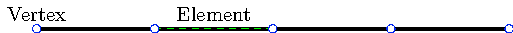
\includegraphics[width = 0.8\linewidth]{figures/1d-mesh.pdf}
    \caption{1D mesh.} % \label{}
\end{figure}
In two and three dimensions, the mesh may be either \textit{structured}
or \textit{unstructured} as shown below. Unstructured meshes typically
consist of triangles (or tetrahedra in 3D).
\begin{figure}[H]
    \centering
    \begin{subfigure}[t]{0.45\textwidth}
        \centering
        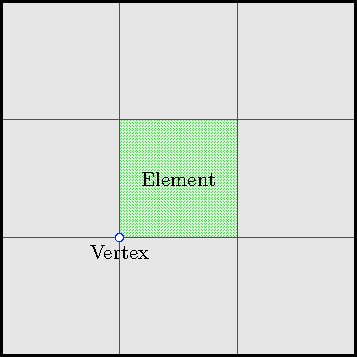
\includegraphics[height = 4cm]{figures/2d-structured-mesh.pdf}
        \caption{2D structured mesh.} % \label{}
    \end{subfigure}
    %
    \begin{subfigure}[t]{0.45\textwidth}
        \centering
        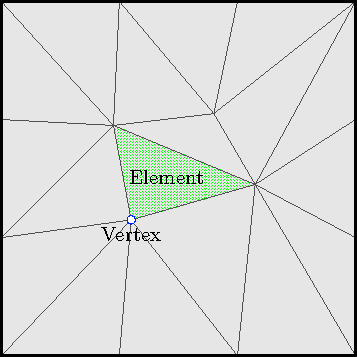
\includegraphics[height = 4cm]{figures/2d-unstructured-mesh.pdf}
        \caption{2D unstructured mesh.} % \label{}
    \end{subfigure}
\end{figure}
The FVM defines:
\begin{itemize}
    \item \textbf{Nodes} \(x_i\), at which the solution is
          approximated by \(u_i\)
    \item \textbf{Control volumes} \(\Omega_i\), over which the
          conservation principle is applied
\end{itemize}
where \(i = 1,\: 2,\: \ldots,\: N\) is the index of the nodes.
There are several ways to define the control volumes. Two common
approaches are:
\begin{itemize}
    \item \textbf{Cell-Centred Control Volumes}: Nodes are positioned
          at the centroids of elements, and control volumes are defined over
          elements.
    \item \textbf{Vertex-Centred Control Volumes}: Nodes are positioned
          at vertices, and control volumes are constructed using the centroids
          of adjacent element boundaries.
\end{itemize}
This is illustrated in 1D and 2D in the following figures.
\begin{figure}[H]
    \centering
    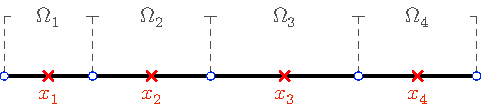
\includegraphics[width = 0.8\linewidth]{figures/1d-cell-centered.pdf}
    \caption{1D mesh with cell-centred control volumes.} % \label{}
\end{figure}
\begin{figure}[H]
    \centering
    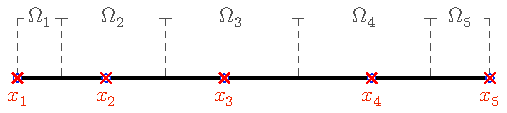
\includegraphics[width = 0.8\linewidth]{figures/1d-vertex-centered.pdf}
    \caption{1D mesh with vertex-centred control volumes.} % \label{}
\end{figure}
\begin{figure}[H]
    \centering
    \begin{subfigure}[t]{0.45\linewidth}
        \centering
        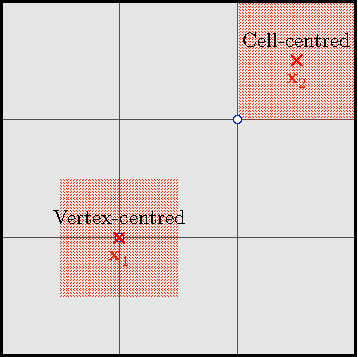
\includegraphics[height = 4cm]{figures/2d-structured-nodes.pdf}
        \caption{2D structured mesh with vertex-/cell- centred control volumes.} % \label{}
    \end{subfigure}
    \begin{subfigure}[t]{0.45\linewidth}
        \centering
        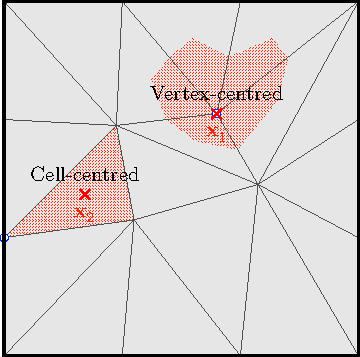
\includegraphics[height = 4cm]{figures/2d-unstructured-nodes.pdf}
        \caption{2D unstructured mesh with vertex-/cell- centred control volumes.} % \label{}
    \end{subfigure}
\end{figure}
For problems in three dimensions using structured meshes, control
volumes are cubes (or rectangular prisms). For unstructured meshes with
control volumes using the cell-centred approach, elements themselves are
used as control volumes. For the vertex-centred approach, control volume
boundaries are defined using the centroids of adjacent element boundaries.
\subsection{General Strategy}
Consider a mesh with \(N\) nodes and \(N\) control volumes:
\begin{enumerate}
    \item Label the nodes \(x_1,\: x_2,\: \ldots,\: x_N\) and the
          unknowns \(u_1,\: u_2,\: \ldots,\: u_N\).
    \item Identify the control volume types (interior nodes when \(2
          \leqslant i \leqslant N-1\), boundary nodes when \(i = 1\) or
          \(i = N\)).
    \item Integrate the transport equation over each control volume and
          apply the Divergence theorem to the flux term.
    \item Incorporate the boundary conditions to approximate/discretise
          all remaining terms.
\end{enumerate}
To discretise the transport equation, let us integrate the transport
equation over each control volume \(\Omega_i\):
\begin{align*}
    \pdv{u}{t} + \symbf{\nabla} \cdot \symbf{q}                                                                  & = R                          \\
    \int_{\Omega_i} \pdv{u}{t} \odif{V} + \int_{\Omega_i} \left( \symbf{\nabla} \cdot \symbf{q} \right) \odif{V} & = \int_{\Omega_i} R \odif{V}
\end{align*}
Applying the divergence theorem to the flux term, we have
\begin{equation*}
    \odv*{\int_{\Omega_i} u \odif{V}}{t} + \int_{\partial \Omega_i} \left( \symbf{q} \cdot \symbf{n} \right) \odif{s} = \int_{\Omega_i} R \odif{V}
\end{equation*}
where \(\partial \Omega_i\) is the control volume boundary of \(\Omega_i\),
and \(\symbf{n}\) is the outward unit vector normal to \(\partial \Omega_i\),
directed out of \(\Omega_i\). Consider the spatial average of \(u\) and
\(R\) over \(\Omega_i\):
\begin{equation*}
    \bar{u}_i = \frac{1}{V_i} \int_{\Omega_i} u \odif{V}, \qquad \bar{R}_i = \frac{1}{V_i} \int_{\Omega_i} R \odif{V}
\end{equation*}
where \(V_i\) is the volume of \(\Omega_i\). Using this quantity, we can
rewrite the transport equation as
\begin{equation*}
    \odv{\bar{u}_i}{t} + \frac{1}{V_i} \int_{\partial \Omega_i} \left( \symbf{q} \cdot \symbf{n} \right) \odif{s} = \bar{R}_i.
\end{equation*}
\section{The Time-Dependent Transport Equation}
Using the discrete approximations \(u_i\) and \(R_i\), at each node
\(x_i\), we arrive at the discrete form of the transport equation:
\begin{equation}
    \boxed{
        \odv{u_i}{t} = - \frac{1}{V_i} \int_{\partial \Omega_i} \left( \symbf{q} \cdot \symbf{n} \right) \odif{s} + R_i.
    }
\end{equation}
Constructing this equation for all \(i\) gives a system of \(N\) ODEs
for the unknowns \(u_i\), in time:
\begin{equation*}
    \odv{\symbf{u}}{t} = \symbf{A} \symbf{u} + \symbf{b}\left( t \right), \qquad \symbf{u}\left( 0 \right) = \symbf{u}^{\left( 0 \right)}
\end{equation*}
where \(\symbf{u} = {\left( u_1,\: \dots,\: u_N \right)}^\top\) is the
numerical solution vector at time \(t\) containing the solution at each
node \(x_i\), and
\(\symbf{u}^{\left( 0 \right)} = {\left( f\left( x_1 \right),\: \dots,\: f\left( x_N \right) \right)}^\top\)
is the initial solution vector.\ \(\symbf{A} \in \R^{N \times N}\) is a
tridiagonal matrix which consists of coefficients obtained via the
finite-difference method, and \(\symbf{b}\left( t \right)\) contains any
time-dependent terms in the transport equation. Note that when the
transport equation is nonlinear, it is expressed as
\begin{equation*}
    \odv{\symbf{u}}{t} = \symbf{G}\left( t,\: \symbf{u}\left( t \right) \right).
\end{equation*}
\section{Time Discretisation}
This time-dependent ODE can be solved using the \(\theta\)-methods.
Consider a sufficiently large final time \(T\), and discretise time
domain into \(M\) time steps of size \(\fdif{t} = T/M = t_{n+1} -
t_n\), such that \(t_n = n \fdif{t}\) for \(n = 0,\: 1,\: \ldots,\:
M\). Then let us split the nonhomogeneous part of this ODE into the
time-independent and time-dependent parts:
\begin{equation*}
    \odv{\symbf{u}}{t} = \symbf{A} \symbf{u} + \symbf{b}_1 + \symbf{b}_2\left( t \right), \qquad \symbf{u}\left( 0 \right) = \symbf{u}^{\left( 0 \right)}.
\end{equation*}
We can then compute \(\symbf{u}^{\left( n \right)} = {\left( u_1^{\left( n \right)},\: \dots,\: u_N^{\left( n \right)} \right)}^\top\),
where \(u_i^{\left( n \right)} \approx u_i\left( t_n \right) = u\left( x_i,\: t_n \right)\),
is the solution at \(x = x_i\) and time \(t = t_n\), using the \(\theta\)-method.

Let us integrate this ODE over the time interval
\(\ointerval{t_n}{t_{n+1}}\):
\begin{align*}
    \int_{t_n}^{t_{n+1}} \odv{\symbf{u}}{t} \odif{t}              & = \int_{t_n}^{t_{n+1}} \left( \symbf{A} \symbf{u} + \symbf{b}_1 + \symbf{b}_2\left( t \right) \right) \odif{t}                                              \\
    \symbf{u}\left( t_{n+1} \right) - \symbf{u}\left( t_n \right) & = \symbf{A} \int_{t_n}^{t_{n+1}} \symbf{u} \odif{t} + \int_{t_n}^{t_{n+1}} \symbf{b}_1 \odif{t} + \int_{t_n}^{t_{n+1}} \symbf{b}_2\left( t \right) \odif{t} \\
    \symbf{u}^{\left( n+1 \right)} - \symbf{u}^{\left( n \right)} & = \symbf{A} \int_{t_n}^{t_{n+1}} \symbf{u} \odif{t} + \symbf{b}_1 \left( t_{n+1} - t_n \right) + \int_{t_n}^{t_{n+1}} \symbf{b}_2\left( t \right) \odif{t}.
\end{align*}
To integrate the time-dependent terms, we will use a \textit{weighted
    \(\theta\) approximation}, where
\begin{equation*}
    \int_{t_n}^{t_{n+1}} f\left( t \right) \odif{t} \approx \fdif{t} \left[ \left( 1 - \theta \right) f\left( t_n \right) + \theta f\left( t_{n+1} \right) \right].
\end{equation*}
Then,
\begin{align*}
    \symbf{u}^{\left( n+1 \right)} - \symbf{u}^{\left( n \right)}                               & = \fdif{t} \symbf{A} \left[ \left( 1 - \theta_1 \right) \symbf{u}^{\left( n \right)} + \theta_1 \symbf{u}^{\left( n+1 \right)} \right] + \symbf{b}_1 \fdif{t} + \fdif{t} \left[ \left( 1 - \theta_2 \right) \symbf{b}_2^{\left( n \right)} + \theta_2 \symbf{b}_2^{\left( n+1 \right)} \right] \\
    \symbf{u}^{\left( n+1 \right)} - \symbf{A} \theta_1 \fdif{t} \symbf{u}^{\left( n+1 \right)} & = \symbf{u}^{\left( n \right)} + \fdif{t} \left( 1 - \theta_1 \right) \symbf{A} \symbf{u}^{\left( n \right)} + \fdif{t} \symbf{b}_1 + \fdif{t} \left[ \left( 1 - \theta_2 \right) \symbf{b}_2^{\left( n \right)} + \theta_2 \symbf{b}_2^{\left( n+1 \right)} \right]
\end{align*}
giving us the time-stepping formula
\begin{equation*}
    \boxed{
    \left( \symbf{I} - \fdif{t} \theta_1 \symbf{A} \right) \symbf{u}^{\left( n+1 \right)} = \left[ \symbf{I} + \fdif{t} \left( 1 - \theta_1 \right) \symbf{A} \right] \symbf{u}^{\left( n \right)} + \fdif{t} \left[ \symbf{b}_1 + \left( 1 - \theta_2 \right) \symbf{b}_2^{\left( n \right)} + \theta_2 \symbf{b}_2^{\left( n+1 \right)} \right]
    }
\end{equation*}
for two choices of \(\theta_1\) and \(\theta_2\). For convenience, we will
write this as
\begin{equation*}
    \tilde{\symbf{A}} \symbf{u}^{\left( n+1 \right)} = \tilde{\symbf{B}} \symbf{u}^{\left( n \right)} + \tilde{\symbf{b}}.
\end{equation*}
Setting \(\theta_1 = \theta_2 = 0\), we obtain the Forward Euler method:
\begin{equation*}
    \symbf{u}^{\left( n+1 \right)} = \left( \symbf{I} + \fdif{t} \symbf{A} \right) \symbf{u}^{\left( n \right)} + \fdif{t} \left( \symbf{b}_1 + \symbf{b}_2^{\left( n \right)} \right)
\end{equation*}
which is an explicit method. Setting \(\theta_1 = \theta_2 = 1\), yields
the Backward Euler method:
\begin{equation*}
    \left( \symbf{I} - \fdif{t} \symbf{A} \right) \symbf{u}^{\left( n+1 \right)} = \symbf{u}^{\left( n \right)} + \fdif{t} \left( \symbf{b}_1 + \symbf{b}_2^{\left( n+1 \right)} \right)
\end{equation*}
while setting \(\theta_1 = \theta_2 = \frac{1}{2}\) gives the Crank-Nicolson
method:
\begin{equation*}
    \left( \symbf{I} - \frac{\fdif{t}}{2} \symbf{A} \right) \symbf{u}^{\left( n+1 \right)} = \left( \symbf{I} + \frac{\fdif{t}}{2} \symbf{A} \right) \symbf{u}^{\left( n \right)} + \frac{\fdif{t}}{2} \left( 2 \symbf{b}_1 + \symbf{b}_2^{\left( n \right)} + \symbf{b}_2^{\left( n+1 \right)} \right)
\end{equation*}
which are both implicit methods. Using different values for \(\theta_1\)
and \(\theta_2\) is also possible, and these methods are known as the
IMEX (Implicit-Explicit) methods.
\subsection{Dirichlet Boundary Conditions}
When a problem defines Dirichlet boundary conditions rather than
Neumann boundary conditions, we must replace the first row of the
matrix \(\tilde{\symbf{A}}\) with \({\left( 1,\: 0,\: \dots,\: 0
\right)} \in \R^{1 \times N}\) and the first element of the RHS vector
\(\tilde{\symbf{b}}\) with the Dirichlet boundary condition to ensure
that the boundary condition is satisfied.
\section{Stability Analysis}
Consider only the interior rows and columns of the result
\begin{equation*}
    \tilde{\symbf{A}} \symbf{u}^{\left( n+1 \right)} = \tilde{\symbf{B}} \symbf{u}^{\left( n \right)} + \tilde{\symbf{b}}
\end{equation*}
where \(\symbf{u} \in \R^{N - 2}\), \(\tilde{\symbf{A}} \in \R^{N - 2 \times N - 2}\),
\(\tilde{\symbf{B}} \in \R^{N - 2 \times N - 2}\), and \(\tilde{\symbf{b}} \in \R^{N - 2}\).
Then let us assume that \(\tilde{\symbf{A}}\) is invertible, so that we
can construct the recurrence relation
\begin{equation*}
    \symbf{u}^{\left( n+1 \right)} = \tilde{\symbf{A}}^{-1} \tilde{\symbf{B}} \symbf{u}^{\left( n \right)} + \tilde{\symbf{A}}^{-1} \tilde{\symbf{b}}.
\end{equation*}
If we consider the homogeneous part of this equation, and let
\(\symbf{T} = \tilde{\symbf{A}}^{-1} \tilde{\symbf{B}}\), we can
analyse the stability of our time discretisation method using
spectral analysis:
\begin{equation*}
    \symbf{u}^{\left( n+1 \right)} = \symbf{T} \symbf{u}^{\left( n \right)}.
\end{equation*}
For a uniform mesh, the matrix \(\symbf{A}\) is tridiagonal with constant
diagonals (or \textit{Toeplitz tridiagonal}):
\begin{equation*}
    \symbf{A} =
    \begin{bmatrix}
        \alpha & \beta  &        &        &        \\
        \gamma & \alpha & \beta  &        &        \\
               & \gamma & \alpha & \ddots &        \\
               &        & \ddots & \ddots & \beta  \\
               &        &        & \gamma & \alpha
    \end{bmatrix}
    .
\end{equation*}
Such a matrix has eigenvalues
\begin{equation*}
    \lambda_i = \alpha + 2 \sqrt{\beta} \sqrt{\gamma} \cos\left( \frac{i \pi}{N+1} \right), \qquad i = 1,\: 2,\: \ldots,\: N-2
\end{equation*}
Consider an error term \(\symbf{\varepsilon}^{\left( 0 \right)}\) present in the
initial solution vector \(\symbf{u}^{\left( 0 \right)}\) at time \(t = 0\).
Then, by the recurrence relation established above,
\begin{align*}
    \symbf{u}^{\left( 1 \right)} & = \symbf{T} \symbf{u}^{\left( 0 \right)} = \symbf{T} \left( \symbf{u}^{\left( 0 \right)} + \symbf{\varepsilon}^{\left( 0 \right)} \right) = \symbf{T} \symbf{u}^{\left( 0 \right)} + \symbf{T} \symbf{\varepsilon}^{\left( 0 \right)}                                \\
    \symbf{u}^{\left( 2 \right)} & = \symbf{T} \symbf{u}^{\left( 1 \right)} = \symbf{T} \left( \symbf{T} \symbf{u}^{\left( 0 \right)} + \symbf{T} \symbf{\varepsilon}^{\left( 0 \right)} \right) = \symbf{T}^2 \symbf{u}^{\left( 0 \right)} + \symbf{T}^2 \symbf{\varepsilon}^{\left( 0 \right)}        \\
                                 & \vdotswithin{=}                                                                                                                                                                                                                                                      \\
    \symbf{u}^{\left( n \right)} & = \symbf{T} \symbf{u}^{\left( n-1 \right)} = \symbf{T} \left( \symbf{T} \symbf{u}^{\left( n-2 \right)} + \symbf{T} \symbf{\varepsilon}^{\left( n-2 \right)} \right) = \symbf{T}^n \symbf{u}^{\left( 0 \right)} + \symbf{T}^n \symbf{\varepsilon}^{\left( 0 \right)}.
\end{align*}
Thus, we must ensure that the error term \(\symbf{T}^n \symbf{\varepsilon}^{\left( 0 \right)}\)
does not grow unbounded as \(n \to M\). This is only possible when the
spectral radius of the matrix \(\symbf{T}\) is smaller than 1, i.e.,
\(\rho\left( \symbf{T} \right) < 1\).

Given that the matrix \(\symbf{A}\) is Toeplitz tridiagonal with
eigenpairs \(\left( \lambda_i,\: \symbf{v}_i \right)\), consider the
eigenvalue problem for the matrix \(\tilde{\symbf{A}}\):
\begin{align*}
    \symbf{A} \symbf{v}_i                                                & = \lambda_i \symbf{v}_i                                                \\
    \left( \fdif{t} \theta_1 \symbf{A} \right) \symbf{v}_i               & = \left( \fdif{t} \theta_1 \lambda_i \right) \symbf{v}_i               \\
    \symbf{v}_i - \left( \fdif{t} \theta_1 \symbf{A} \right) \symbf{v}_i & = \symbf{v}_i - \left( \fdif{t} \theta_1 \lambda_i \right) \symbf{v}_i \\
    \left( \symbf{I} - \fdif{t} \theta_1 \symbf{A} \right) \symbf{v}_i   & = \left( 1 - \fdif{t} \theta_1 \lambda_i \right) \symbf{v}_i           \\
    \tilde{\symbf{A}} \symbf{v}_i                                        & = \psi_i \symbf{v}_i.
\end{align*}
Similarly for the matrix \(\tilde{\symbf{B}}\):
\begin{align*}
    \symbf{A} \symbf{v}_i                                                                   & = \lambda_i \symbf{v}_i                                                                   \\
    \left( \fdif{t} \left( 1 - \theta_1 \right) \symbf{A} \right) \symbf{v}_i               & = \left( \fdif{t} \left( 1 - \theta_1 \right) \lambda_i \right) \symbf{v}_i               \\
    \symbf{v}_i + \left( \fdif{t} \left( 1 - \theta_1 \right) \symbf{A} \right) \symbf{v}_i & = \symbf{v}_i + \left( \fdif{t} \left( 1 - \theta_1 \right) \lambda_i \right) \symbf{v}_i \\
    \left( \symbf{I} + \fdif{t} \left( 1 - \theta_1 \right) \symbf{A} \right) \symbf{v}_i   & = \left( 1 + \fdif{t} \left( 1 - \theta_1 \right) \lambda_i \right) \symbf{v}_i           \\
    \tilde{\symbf{B}} \symbf{v}_i                                                           & = \phi_i \symbf{v}_i.
\end{align*}
Thus, the eigenvalues of the matrices \(\tilde{\symbf{A}}\) and
\(\tilde{\symbf{B}}\) are \(\left( 1 - \fdif{t} \theta_1 \lambda_i \right)\)
and \(\left( 1 + \fdif{t} \left( 1 - \theta_1 \right) \lambda_i \right)\),
respectively, so that the eigenvalues of the matrix \(\symbf{T}\) are
given by the ratio of the eigenvalues of the matrices \(\tilde{\symbf{A}}\)
and \(\tilde{\symbf{B}}\):
\begin{align*}
    \tilde{\symbf{A}}^{-1} \tilde{\symbf{B}} \symbf{v}_i & = \tilde{\symbf{A}}^{-1} \left( \phi_i \symbf{v}_i \right)                                                \\
    \symbf{T} \symbf{v}_i                                & = \frac{1}{\psi_i} \phi_i \symbf{v}_i                                                                     \\
    \symbf{T} \symbf{v}_i                                & = \frac{1 + \fdif{t} \left( 1 - \theta_1 \right) \lambda_i}{1 - \fdif{t} \theta_1 \lambda_i} \symbf{v}_i.
\end{align*}
We can now find a lower bound for the spectral radius through some
algebra:
\begin{align*}
    \rho\left( \symbf{T} \right) & = \max \abs*{\frac{1 + \fdif{t} \left( 1 - \theta_1 \right) \lambda_i}{1 - \fdif{t} \theta_1 \lambda_i}}                                                                                                                                                                                                             \\
                                 & = \max \abs*{\frac{1 + \fdif{t} \lambda_i - \fdif{t} \theta_1 \lambda_i}{1 - \fdif{t} \theta_1 \lambda_i}}                                                                                                                                                                                                           \\
                                 & = \max \abs*{1 + \frac{\fdif{t} \lambda_i}{1 - \fdif{t} \theta_1 \lambda_i}}.                                                                                                                                                                                                                                        \\
                                 & = \max \abs*{1 + \frac{\fdif{t} \left( \alpha + 2 \sqrt{\beta \gamma} \cos\left( \frac{i \pi}{N+1} \right) \right)}{1 - \fdif{t} \theta_1 \left( \alpha + 2 \sqrt{\beta \gamma} \cos\left( \frac{i \pi}{N+1} \right) \right)}}                                                                                       \\
                                 & = \max \abs*{1 + \frac{\fdif{t} \left( \alpha + 2 \sqrt{\beta \gamma} - 4 \sqrt{\beta \gamma} \sin^2\left( \frac{i \pi}{2 \left( N+1 \right)} \right) \right)}{1 - \fdif{t} \theta_1 \left( \alpha + 2 \sqrt{\beta \gamma} - 4 \sqrt{\beta \gamma} \sin^2\left( \frac{i \pi}{2 \left( N+1 \right)} \right) \right)}} \\
                                 & \geqslant \abs*{1 + \frac{\fdif{t} \left( \alpha + 2 \sqrt{\beta \gamma} \right)}{1 - \fdif{t} \theta_1 \left( \alpha + 2 \sqrt{\beta \gamma} \right)}}
\end{align*}
Therefore,
\begin{equation*}
    \abs*{1 + \frac{\fdif{t} \left( \alpha + 2 \sqrt{\beta \gamma} \right)}{1 - \fdif{t} \theta_1 \left( \alpha + 2 \sqrt{\beta \gamma} \right)}} \leqslant \rho\left( \symbf{T} \right) < 1 \implies -1 < 1 + \frac{\fdif{t} \left( \alpha + 2 \sqrt{\beta \gamma} \right)}{1 - \fdif{t} \theta_1 \left( \alpha + 2 \sqrt{\beta \gamma} \right)} < 1.
\end{equation*}
We need only to consider the upper bound for \(\fdif{t}\), as the lower
bound is trivially satisfied for all \(\fdif{t} > 0\). Thus, we have
\begin{align*}
    -1                                                                                   & < 1 + \frac{\fdif{t} \left( \alpha + 2 \sqrt{\beta \gamma} \right)}{1 - \fdif{t} \theta_1 \left( \alpha + 2 \sqrt{\beta \gamma} \right)} \\
    -2 + 2 \fdif{t} \theta_1 \left( \alpha + 2 \sqrt{\beta \gamma} \right)               & < \fdif{t} \left( \alpha + 2 \sqrt{\beta \gamma} \right)                                                                                 \\
    \fdif{t} \left( \alpha + 2 \sqrt{\beta \gamma} \right) \left( 2 \theta_1 - 1 \right) & < 2                                                                                                                                      \\
    \fdif{t}                                                                             & > \frac{2}{\left( \alpha + 2 \sqrt{\beta \gamma} \right) \left( 2 \theta_1 - 1 \right)}.
\end{align*}
\section{Monotonicity}
For a numerical solution to remain physically meaningful, it must be
monotonic. That is, in the absence of a reaction/source term, an
increase in the solution at any neighbouring node must not cause a
decrease in the solution at the current node. Failure to observe this
may result in oscillations in the numerical solution. Consider the
diagonal and off-diagonal parts of the LHS of the time-discretisation:
\begin{align*}
    \symbf{I} - \fdif{t} \theta_1 \symbf{A} & =
    \begin{bmatrix}
        1 - \fdif{t} \theta_1 \alpha & -\fdif{t} \theta_1 \beta     &                           &                              \\
        -\fdif{t} \theta_1 \gamma    & 1 - \fdif{t} \theta_1 \alpha & \ddots                    &                              \\
                                     & \ddots                       & \ddots                    & -\fdif{t} \theta_1 \beta     \\
                                     &                              & -\fdif{t} \theta_1 \gamma & 1 - \fdif{t} \theta_1 \alpha
    \end{bmatrix}
    \\
                                            & =
    \begin{bmatrix}
        1 - \fdif{t} \theta_1 \alpha &                              &        &                              \\
                                     & 1 - \fdif{t} \theta_1 \alpha &        &                              \\
                                     &                              & \ddots &                              \\
                                     &                              &        & 1 - \fdif{t} \theta_1 \alpha
    \end{bmatrix}
    +
    \begin{bmatrix}
        0                         & -\fdif{t} \theta_1 \beta &                           &                          \\
        -\fdif{t} \theta_1 \gamma & 0                        & \ddots                    &                          \\
                                  & \ddots                   & \ddots                    & -\fdif{t} \theta_1 \beta \\
                                  &                          & -\fdif{t} \theta_1 \gamma & 0
    \end{bmatrix}
    \\
                                            & = \left( 1 - \fdif{t} \theta_1 \alpha \right) \symbf{I} +
    \begin{bmatrix}
        0                         & -\fdif{t} \theta_1 \beta &                           &                          \\
        -\fdif{t} \theta_1 \gamma & 0                        & \ddots                    &                          \\
                                  & \ddots                   & \ddots                    & -\fdif{t} \theta_1 \beta \\
                                  &                          & -\fdif{t} \theta_1 \gamma & 0
    \end{bmatrix}
    .
\end{align*}
The off-diagonal part of the matrix can be expressed as the difference
of the original matrix and a diagonal matrix:
\begin{align*}
    \begin{bmatrix}
        0                         & -\fdif{t} \theta_1 \beta &                           &                          \\
        -\fdif{t} \theta_1 \gamma & 0                        & \ddots                    &                          \\
                                  & \ddots                   & \ddots                    & -\fdif{t} \theta_1 \beta \\
                                  &                          & -\fdif{t} \theta_1 \gamma & 0
    \end{bmatrix}
     & = \symbf{I} - \fdif{t} \theta_1 \symbf{A} - \left( 1 - \fdif{t} \theta_1 \alpha \right) \symbf{I} \\
     & = \symbf{I} - \fdif{t} \theta_1 \symbf{A} - \symbf{I} + \fdif{t} \theta_1 \alpha \symbf{I}        \\
     & = -\fdif{t} \theta_1 \left( \symbf{A} - \alpha \symbf{I} \right).
\end{align*}
Therefore,
\begin{align*}
    \left( \symbf{I} - \fdif{t} \theta_1 \symbf{A} \right) \symbf{u}^{\left( n+1 \right)}                                                                               & = \left[ \symbf{I} + \fdif{t} \left( 1 - \theta_1 \right) \symbf{A} \right] \symbf{u}^{\left( n \right)} + \tilde{\symbf{b}}                                                                                                 \\
    \left[ \left( 1 - \fdif{t} \theta_1 \alpha \right) \symbf{I} - \fdif{t} \theta_1 \left( \symbf{A} - \alpha \symbf{I} \right) \right] \symbf{u}^{\left( n+1 \right)} & = \left[ \symbf{I} + \fdif{t} \left( 1 - \theta_1 \right) \symbf{A} \right] \symbf{u}^{\left( n \right)} + \tilde{\symbf{b}}                                                                                                 \\
    \left( 1 - \fdif{t} \theta_1 \alpha \right) \symbf{u}^{\left( n+1 \right)}                                                                                          & = \fdif{t} \theta_1 \left( \symbf{A} - \alpha \symbf{I} \right) \symbf{u}^{\left( n+1 \right)} + \left[ \symbf{I} + \fdif{t} \left( 1 - \theta_1 \right) \symbf{A} \right] \symbf{u}^{\left( n \right)} + \tilde{\symbf{b}}.
\end{align*}
Let us consider the individual elements of the two matrix terms on the RHS:
\begin{align*}
    \fdif{t} \theta_1 \left( \symbf{A} - \alpha \symbf{I} \right) & = \fdif{t} \theta_1
    \begin{bmatrix}
        0      & \beta  &        &       \\
        \gamma & 0      & \ddots &       \\
               & \ddots & \ddots & \beta \\
               &        & \gamma & 0
    \end{bmatrix}
    ,
    \\
    \symbf{I} + \fdif{t} \left( 1 - \theta_1 \right) \symbf{A}    & = \symbf{I} + \fdif{t} \left( 1 - \theta_1 \right)
    \begin{bmatrix}
        \alpha & \beta  &        &        \\
        \gamma & \alpha & \ddots &        \\
               & \ddots & \ddots & \beta  \\
               &        & \gamma & \alpha
    \end{bmatrix}
    .
\end{align*}
For the solution of this equation to be monotonic, all coefficients of
\(\symbf{u}\) must be non-negative:
\begin{gather*}
    1 - \fdif{t} \theta_1 \alpha \geqslant 0, \\
    \fdif{t} \theta_1 \beta \geqslant 0, \qquad \fdif{t} \theta_1 \gamma \geqslant 0, \\
    1 + \fdif{t} \left( 1 - \theta_1 \right) \alpha \geqslant 0, \quad 1 + \fdif{t} \left( 1 - \theta_1 \right) \beta \geqslant 0, \quad 1 + \fdif{t} \left( 1 - \theta_1 \right) \gamma \geqslant 0.
\end{gather*}
From the second row, both \(\beta\) and \(\gamma\) must be non-negative.
Therefore, the time step \(\fdif{t}\) must satisfy the following
conditions:
\begin{equation*}
    \fdif{t} \geqslant \frac{1}{\theta_1 \alpha}, \quad \fdif{t} \geqslant \frac{1}{\left( 1 - \theta_1 \right) \alpha}, \quad \fdif{t} \geqslant \frac{1}{\left( 1 - \theta_1 \right) \beta}, \quad \fdif{t} \geqslant \frac{1}{\left( 1 - \theta_1 \right) \gamma}.
\end{equation*}
\section{Finite Volume Method in 1D}
Let us define the following geometric quantities (for the
vertex-centred control volume strategy):
\begin{figure}[H]
    \centering
    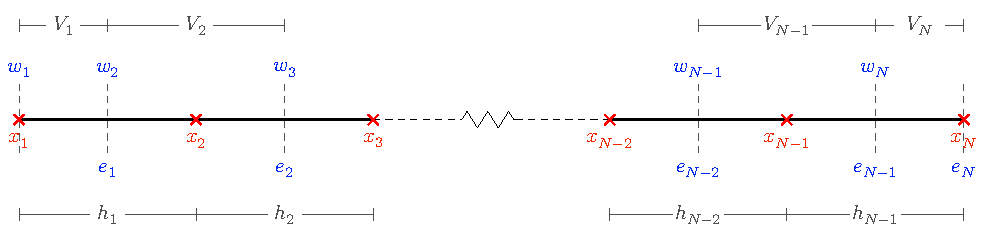
\includegraphics[width = \linewidth]{figures/1d-fvm.pdf}
    \caption{1D FVM.} % \label{}
\end{figure}
where
\begin{itemize}
    \item \(\Omega = \ointerval{x_1}{x_N}\)
    \item \(\Omega_i = \ointerval{w_i}{e_i}\) is the control volume for node \(i\)
    \item \(h_i\) is the spacing between nodes \(i\) and \(i + 1\)
          \begin{equation*}
              h_i = x_{i+1} - x_i \quad \text{for \(i = 1,\: \ldots,\: N-1\)}
          \end{equation*}
    \item \(V_i\) is the volume of control volume \(\Omega_i\)
          \begin{equation*}
              V_i =
              \begin{cases}
                  \displaystyle \frac{h_1}{2},           & i = 1                       \\
                  \displaystyle \frac{h_{i-1} + h_i}{2}, & 2 \leqslant i \leqslant N-1 \\
                  \displaystyle \frac{h_{N-1}}{2},       & i = N
              \end{cases}
          \end{equation*}
    \item \(w_i\) and \(e_i\) are the west and east boundaries of
          control volume \(\Omega_i\)
          \begin{align*}
              w_i & =
              \begin{cases}
                  \displaystyle x_1,                     & i = 1                     \\
                  \displaystyle \frac{x_{i-1} + x_i}{2}, & 2 \leqslant i \leqslant N
              \end{cases}
              \\
              e_i & =
              \begin{cases}
                  \displaystyle \frac{x_i + x_{i+1}}{2}, & 1 \leqslant i \leqslant N-1 \\
                  \displaystyle x_N,                     & i = N
              \end{cases}
          \end{align*}
\end{itemize}
Then, if we integrate over all control volumes \(\Omega_i\) in 1D, the
spatial averages simplify to:
\begin{equation*}
    \bar{u}_i = \frac{1}{V_i} \int_{w_i}^{e_i} u \odif{x}, \qquad \bar{R}_i = \frac{1}{V_i} \int_{w_i}^{e_i} R \odif{x}
\end{equation*}
likewise, the flux term becomes,
\begin{align*}
    \int_{\Omega_i} \left( \symbf{\nabla} \cdot \symbf{q} \right) \odif{V} & = \int_{w_i}^{e_i} \pdv{q}{x} \odif{x} \\
                                                                           & = q_{e_i} - q_{w_i}
\end{align*}
so that
\begin{equation*}
    \odv{u_i}{t} = \frac{1}{V_i} \left( q_{w_i} - q_{e_i} \right) + R_i.
\end{equation*}
\subsection{Finite Differences}
\subsubsection{Internal Nodes}
We can apply the finite-difference method at internal nodes, using:
\begin{align*}
    u\left( w_i,\: t \right) & = \left( 1 - \sigma \right)  u_{i-1} + \sigma u_i & \pdv{u}{x}\left( w_i,\: t \right) & = \frac{u_i - u_{i-1}}{h_{i-1}} &  & \text{(west node)} \\
    u\left( e_i,\: t \right) & = \left( 1 - \sigma \right)  u_i + \sigma u_{i+1} & \pdv{u}{x}\left( e_i,\: t \right) & = \frac{u_{i+1} - u_i}{h_i}     &  & \text{(east node)}
\end{align*}
for weights \(0 \leqslant \sigma \leqslant 1\). The choice
\(\sigma = 1/2\) is known as \textit{averaging}, as it produces
\begin{equation*}
    u\left( w_i,\: t \right) = \frac{u_{i-1} + u_i}{2}, \qquad u\left( e_i,\: t \right) = \frac{u_i + u_{i+1}}{2}.
\end{equation*}
When \(v > 0\), then the flow is from left to right, and we choose \(\sigma
= 0\), so that
\begin{equation*}
    u\left( w_i,\: t \right) \approx u_{i-1}, \qquad u\left( e_i,\: t \right) \approx u_i.
\end{equation*}
When \(v < 0\), then the flow is from right to left, and we choose
\(\sigma = 1\), so that
\begin{equation*}
    u\left( w_i,\: t \right) \approx u_i, \qquad u\left( e_i,\: t \right) \approx u_{i+1}.
\end{equation*}
This is known as \textit{upwinding}. Numerical solutions obtained using
upwinding exhibit \textit{numerical diffusion} or \textit{false diffusion}
as we can rewrite the diffusivity in the upwinding method using the
diffusivity from the averaging method:
\(D_{\text{upwinding}} = D_{\text{avg}} + c\), where \(c\) is some
constant made up of the model parameters.
\subsubsection{Boundary Nodes}
At boundary nodes, we can use boundary conditions to approximate
\(\pdv{u}{x}\) at the boundaries:
\begin{align*}
    \pdv{u}{x}\left( w_1,\: t \right) & = \pdv{u}{x}\left( 0,\: t \right) & \pdv{u}{x}\left( e_1,\: t \right) & = \frac{u_2 - u_1}{h_1}           &  & \text{(left boundary)}  \\
    \pdv{u}{x}\left( w_N,\: t \right) & = \frac{u_N - u_{N-1}}{h_{N-1}}   & \pdv{u}{x}\left( e_N,\: t \right) & = \pdv{u}{x}\left( L,\: t \right) &  & \text{(right boundary)}
\end{align*}
\subsubsection{Nonlinear Diffusivity}
If the diffusivity is a nonlinear function of \(u\), then we can use
the following averaging approximations:
\begin{align*}
    D\left( u\left( x_i,\: t \right) \right) & = D\left( u_i \right)                                     &  & \text{(current node)} \\
    D\left( u\left( w_i,\: t \right) \right) & = \frac{D\left( u_{i-1} \right) + D\left( u_i \right)}{2} &  & \text{(west node)}    \\
    D\left( u\left( e_i,\: t \right) \right) & = \frac{D\left( u_i \right) + D\left( u_{i+1} \right)}{2} &  & \text{(east node)}
\end{align*}
\subsection{Time Discretisation}
We can compute \(u_i^{\left( n \right)} = u_i\left( t_n \right) =
u\left( x_i,\: t_n \right)\) by integrating the above ODE over the time
interval \(\ointerval{t_n}{t_{n+1}}\):
\begin{align*}
    \int_{t_n}^{t_{n+1}} \odv{u_i}{t} \odif{t}        & = \int_{t_n}^{t_{n+1}} \left( \frac{1}{V_i} \left( q_{w_i} - q_{e_i} \right) + R_i \right) \odif{t} \\
    u_i\left( t_{n+1} \right) - u_i\left( t_n \right) & = \frac{1}{V_i} \int_{t_n}^{t_{n+1}} q_{w_i} - q_{e_i} \odif{t} + \int_{t_n}^{t_{n+1}} R_i \odif{t} \\
    u_i^{\left( n+1 \right)} - u_i^{\left( n \right)} & =
    \begin{aligned}[t]
         & {}\frac{\fdif{t}}{V_i} \left[ \left( 1 - \theta_1 \right) \left( q_{w_i}^{\left( n \right)} - q_{e_i}^{\left( n \right)} \right) + \theta_1 \left( q_{w_i}^{\left( n+1 \right)} - q_{e_i}^{\left( n+1 \right)} \right) \right] \\
         & {}+ \fdif{t} \left[ \left( 1 - \theta_2 \right) R_i^{\left( n \right)} + \theta_2 R_i^{\left( n+1 \right)} \right].
    \end{aligned}
\end{align*}
\part{Newton Methods}
Consider the nonlinear form of the time-dependent ODE, which arises
when \(D\) or \(R\) are nonlinear functions of \(u\):
\begin{equation*}
    \odv{u}{t} = \symbf{G}\left( u \right).
\end{equation*}
If we were to use the \(\theta\)-method, we find that the solution requires
iterating over the solution \(M-2\) times:
\begin{equation*}
    \symbf{u}^{\left( n+1 \right)} - \symbf{u}^{\left( n \right)} = \fdif{t} \left[ \theta_1 \symbf{G}\left( \symbf{u}^{\left( n+1 \right)} \right) + \left( 1 - \theta_1 \right) \symbf{G}\left( \symbf{u}^{\left( n \right)} \right) \right].
\end{equation*}
Let us consider an iterative approach where we approximate the solution
\(\symbf{u}^{\left( n+1 \right)}\) at every time step \(n\) by finding
the root of the vector function:
\begin{align*}
    \symbf{x} - \symbf{u}^{\left( n \right)} - \fdif{t} \left[ \theta_1 \symbf{G}\left( \symbf{x} \right) + \left( 1 - \theta_1 \right) \symbf{G}\left( \symbf{u}^{\left( n \right)} \right) \right] & = \symbf{0}  \\
    \symbf{F}\left( \symbf{x} \right)                                                                                                                                                                & = \symbf{0}.
\end{align*}
The initial guess for this algorithm will be the solution at the previous
time step:
\begin{equation*}
    \symbf{x}^{\left( 0 \right)} = \symbf{u}^{\left( n \right)}
\end{equation*}
so that when Newton's method converges, the root after \(k\) iterations
approximates the solution at the next time step:
\begin{equation*}
    \symbf{u}^{\left( n+1 \right)} = \symbf{x}^{\left( k \right)}.
\end{equation*}
This is repeated until an approximate solution is obtained at each time
step.
\section{Newton's Method}
Newton's method is an iterative method for finding the roots of a
nonlinear function.
\subsection{Scalar Function}
Given a scalar function \(f\left( x \right)\), we can approximate the
root of this function by linearising the function about a guess
\(x^{\left( k \right)}\):
\begin{align*}
    f\left( x \right)      & \approx f\left( x^{\left( k \right)} \right) + f'\left( x^{\left( k \right)} \right) \left( x - x^{\left( k \right)} \right) \\
    0                      & \approx f\left( x^{\left( k \right)} \right) + f'\left( x^{\left( k \right)} \right) \left( x - x^{\left( k \right)} \right) \\
    x^{\left( k+1 \right)} & = x^{\left( k \right)} - \frac{f\left( x^{\left( k \right)} \right)}{f'\left( x^{\left( k \right)} \right)}.
\end{align*}
\subsection{Vector Function}
Given a system of nonlinear equations, expressed by the vector function
\(\symbf{F}\left( \symbf{x} \right)\), we can use the same
linearisation technique to find the root of this function:
\begin{align*}
    \begin{bmatrix}
        F_1\left( \symbf{x} \right) \\
        F_2\left( \symbf{x} \right) \\
        \vdots                      \\
        F_n\left( \symbf{x} \right)
    \end{bmatrix}
                                      & \approx
    \begin{bmatrix}
        F_1\left( \symbf{x}^{\left( k \right)} \right) \\
        F_2\left( \symbf{x}^{\left( k \right)} \right) \\
        \vdots                                         \\
        F_n\left( \symbf{x}^{\left( k \right)} \right)
    \end{bmatrix}
    +
    \begin{bmatrix}
        \symbf{\nabla} F_1\left( \symbf{x}^{\left( k \right)} \right)^\top \\
        \symbf{\nabla} F_2\left( \symbf{x}^{\left( k \right)} \right)^\top \\
        \vdots                                                             \\
        \symbf{\nabla} F_n\left( \symbf{x}^{\left( k \right)} \right)^\top
    \end{bmatrix}
    \left( \symbf{x} - \symbf{x}^{\left( k \right)} \right)                                                                                                                                                         \\
    \symbf{F}\left( \symbf{x} \right) & \approx \symbf{F}\left( \symbf{x}^{\left( k \right)} \right) + \symbf{J}\left( \symbf{x}^{\left( k \right)} \right) \left( \symbf{x} - \symbf{x}^{\left( k \right)} \right) \\
    \symbf{0}                         & \approx \symbf{F}\left( \symbf{x}^{\left( k \right)} \right) + \symbf{J}\left( \symbf{x}^{\left( k \right)} \right) \left( \symbf{x} - \symbf{x}^{\left( k \right)} \right) \\
    \symbf{x}^{\left( k+1 \right)}    & = \symbf{x}^{\left( k \right)} - \symbf{J}\left( \symbf{x}^{\left( k \right)} \right)^{-1} \symbf{F}\left( \symbf{x}^{\left( k \right)} \right).
\end{align*}
To avoid the matrix inverse, we can instead use the update rule
\begin{equation*}
    \symbf{x}^{\left( k+1 \right)} = \symbf{x}^{\left( k \right)} + \symbf{\delta} \symbf{x}^{\left( k \right)}
\end{equation*}
where \(\symbf{\delta} \symbf{x}^{\left( k \right)}\) is the solution to
the linear system
\begin{equation*}
    \symbf{J}\left( \symbf{x}^{\left( k \right)} \right) \left( \symbf{\delta} \symbf{x}^{\left( k \right)} \right) = -\symbf{F}\left( \symbf{x}^{\left( k \right)} \right).
\end{equation*}
The vector \(\symbf{\delta} \symbf{x}^{\left( k \right)}\) is known as
the \textbf{Newton correction}. We can define the stopping criterion for
the Newton method as
\begin{equation*}
    \norm*{\symbf{F}\left( \symbf{x}^{\left( k + 1 \right)} \right)} \leqslant \text{rtol}\ \norm*{\symbf{F}\left( \symbf{x}^{\left( 0 \right)} \right)} + \text{atol}.
\end{equation*}
\section{Modified Newton Methods}
\subsection{Chord Method}
To avoid the computation of the Jacobian at every iteration, we can
compute the Jacobian at only the first iteration:
\begin{equation*}
    \symbf{x}^{\left( k+1 \right)} = \symbf{x}^{\left( k \right)} - \symbf{J}\left( \symbf{x}^{\left( 0 \right)} \right)^{-1} \symbf{F}\left( \symbf{x}^{\left( k \right)} \right).
\end{equation*}
Using the alternate form shown in the previous section, we can write
this as:
\begin{equation*}
    \symbf{x}^{\left( k+1 \right)} = \symbf{x}^{\left( k \right)} + \symbf{\delta} \symbf{x}^{\left( 0 \right)}
\end{equation*}
where \(\symbf{\delta} \symbf{x}^{\left( 0 \right)}\) is the solution to
the linear system
\begin{equation*}
    \symbf{J}\left( \symbf{x}^{\left( 0 \right)} \right) \left( \symbf{\delta} \symbf{x}^{\left( 0 \right)} \right) = -\symbf{F}\left( \symbf{x}^{\left( k \right)} \right).
\end{equation*}
\subsection{Shamanskii Method}
Alternatively, the Jacobian matrix may be \textit{periodically} updated
every \(m\) iterations. The Shamanskii method is the most general form
of Newton's method, where the original form of Newton's method is
recovered when \(m = 1\), and the Chord method is recovered when \(m
\to \infty\).
\section{Convergence Theory}
The sequence \(\left\{ \symbf{x}^{\left( k \right)} \right\}_{k =
0}^\infty\) converges with limit \(\symbf{x}^\ast\) if:
\begin{equation*}
    \lim_{k \to \infty} \norm*{\symbf{x}^{\left( k \right)} - \symbf{x}^\ast} = 0.
\end{equation*}
The following definitions and theorems will be used throughout this
section to discuss the convergence of the Newton methods discussed
previously.
\subsection{Convergent Sequences}
\begin{definition}[Convergent sequence]
    A sequence \(\left\{ \symbf{x}^{\left( k \right)} \right\}_{k = 0}^\infty\)
    of vectors in \(\R^n\) is convergent with limit \(\symbf{x}^\ast\)
    if for every \(\epsilon > 0\), there exists an integer \(M\) such that
    \begin{equation*}
        \norm*{\symbf{x}^{\left( k \right)} - \symbf{x}^\ast} < \epsilon,
    \end{equation*}
    for all \(k > M\).
\end{definition}
\begin{definition}[Cauchy sequence]
    A sequence \(\left\{ \symbf{x}^{\left( k \right)} \right\}_{k = 0}^\infty\)
    of vectors in \(\R^n\) is a \textbf{Cauchy sequence} if for every
    \(\epsilon > 0\), there exists an integer \(M\) such that
    \begin{equation*}
        \norm*{\symbf{x}^{\left( k \right)} - \symbf{x}^{\left( m \right)}} < \epsilon,
    \end{equation*}
    for all \(k,m > M\).
\end{definition}
A sequence of vectors in \(\R^n\) is Cauchy if and only if it converges.
\begin{definition}[Rate of Convergence]
    Let \(\left\{ \symbf{x}^{\left( k \right)} \right\}_{k = 0}^\infty\)
    be a convergent sequence of vectors in \(\R^n\) with limit \(\symbf{x}^\ast\).
    The sequence converges
    \begin{itemize}
        \item \textbf{quadratically} if there exists a \(K > 0\) such that
              \begin{equation*}
                  \norm*{\symbf{x}^{\left( k+1 \right)} - \symbf{x}^\ast} \leqslant K \norm*{\symbf{x}^{\left( k \right)} - \symbf{x}^\ast}^2
              \end{equation*}
        \item \textbf{superlinearly} with order \(\alpha \in \ointerval{1}{2}\) if there exists a \(K > 0\) such that
              \begin{equation*}
                  \norm*{\symbf{x}^{\left( k+1 \right)} - \symbf{x}^\ast} \leqslant K \norm*{\symbf{x}^{\left( k \right)} - \symbf{x}^\ast}^\alpha
              \end{equation*}
        \item \textbf{linearly} with factor \(\sigma \in \ointerval{0}{1}\) if
              \begin{equation*}
                  \norm*{\symbf{x}^{\left( k+1 \right)} - \symbf{x}^\ast} \leqslant \alpha \norm*{\symbf{x}^{\left( k \right)} - \symbf{x}^\ast}
              \end{equation*}
    \end{itemize}
    for a sufficiently large \(k\).
\end{definition}
\begin{theorem}
    Let \(\symbf{F} :  D \to \R^n\) be differentiable on an open subset
    \(D \subset \R^n\) and let \(\symbf{x} \in D\). Then, for any nonzero
    vector \(\symbf{h}\), such that \(\symbf{x} + \symbf{h} \in D\), we
    have
    \begin{equation*}
        \symbf{F}\left( \symbf{x} + \symbf{h} \right) = \symbf{F}\left( \symbf{x} \right) + \int_0^1 \symbf{J}\left( \symbf{x} + t \symbf{h} \right) \symbf{h} \odif{t}
    \end{equation*}
    where \(\symbf{J}\) is the Jacobian matrix of \(\symbf{F}\).
\end{theorem}
\begin{proof}
    Consider the parameterisation \(\symbf{F}\left( \symbf{x} + t \symbf{h} \right)\),
    then,
    \begin{equation*}
        \pdv{\symbf{F}\left( \symbf{x} + t \symbf{h} \right)}{t} = \pdv{\symbf{F}\left( \symbf{x} + t \symbf{h} \right)}{\left( \symbf{x} + t \symbf{h} \right)} \pdv{\left( \symbf{x} + t \symbf{h} \right)}{t} = \symbf{J}\left( \symbf{x} + t \symbf{h} \right) \symbf{h}.
    \end{equation*}
    We can then integrate this result between \(0\) and \(1\):
    \begin{align*}
        \int_0^1 \pdv*{\symbf{F}\left( \symbf{x} + t \symbf{h} \right)}{t} \odif{t}       & = \int_0^1 \symbf{J}\left( \symbf{x} + t \symbf{h} \right) \symbf{h} \odif{t}                                      \\
        \left[ \symbf{F}\left( \symbf{x} + t \symbf{h} \right) \right]_0^1                & = \int_0^1 \symbf{J}\left( \symbf{x} + t \symbf{h} \right) \symbf{h} \odif{t}                                      \\
        \symbf{F}\left( \symbf{x} + \symbf{h} \right) - \symbf{F}\left( \symbf{x} \right) & = \int_0^1 \symbf{J}\left( \symbf{x} + t \symbf{h} \right) \symbf{h} \odif{t}                                      \\
        \symbf{F}\left( \symbf{x} + \symbf{h} \right)                                     & = \symbf{F}\left( \symbf{x} \right) + \int_0^1 \symbf{J}\left( \symbf{x} + t \symbf{h} \right) \symbf{h} \odif{t}.
    \end{align*}
\end{proof}
\subsection{Lipschitz Continuity}
\begin{definition}[Lipschitz continuous]
    Let \(D \in \R^n\) and \(\symbf{J} : D \to \R^{n \times n}\).
    \(\symbf{J}\) is \textbf{Lipschitz continuous} on \(D\), with
    \textbf{Lipschitz constant} \(\gamma\) if
    \begin{equation*}
        \norm*{\symbf{J}\left( \symbf{x} \right) - \symbf{J}\left( \symbf{y} \right)} \leqslant \gamma \norm*{\symbf{x} - \symbf{y}}, \quad \forall \symbf{x}, \symbf{y} \in D.
    \end{equation*}
    We can denote this as \(\symbf{J} \in \mathrm{Lip}_\gamma\left( D \right)\).
\end{definition}
Using this definition, the \textbf{Standard Assumptions of Newton's Method}
can be described as follows:
\begin{enumerate}
    \item \(\symbf{F}\left( \symbf{x} \right) = \symbf{0}\) has a solution \(\symbf{x}^\ast\) on \(D \subset \R^n\).
    \item \(\symbf{J} \in \mathrm{Lip}_\gamma\left( D \right)\).
    \item \(\symbf{J}\left( \symbf{x} \right)\) is nonsingular and \(\norm*{\symbf{J}\left( \symbf{x} \right)} \leqslant \beta\) for all \(\symbf{x} \in D\).
\end{enumerate}
\begin{theorem}
    Let \(\symbf{F} : D \to \R^n\) for some open subset \(D \subset \R^n\)
    and let the standard assumptions hold. Then, there exists some \(\delta\)
    such that given \(\symbf{x}^{\left( 0 \right)} \in D\) with
    \(\norm*{\symbf{x}^{\left( 0 \right)} - \symbf{x}^\ast} < \delta\),
    the Newton iteration
    \begin{equation*}
        \symbf{x}^{\left( k + 1 \right)} = \symbf{x}^{\left( k \right)} - \symbf{J}\left( \symbf{x}^{\left( k \right)} \right)^{-1} \symbf{F}\left( \symbf{x}^{\left( k \right)} \right)
    \end{equation*}
    satisfies \(\norm*{\symbf{x}^{\left( k \right)} - \symbf{x}^\ast} < \delta\)
    for all \(k\), and converges quadratically to \(\symbf{x}^\ast\).
\end{theorem}
\begin{lemma}
    Let \(\symbf{F} : D \to \R^n\) for some open subset \(D \subset \R^n\)
    and let the standard assumptions hold. Then, the local linear model
    \begin{equation*}
        \symbf{M}_k\left( \symbf{x} \right) = \symbf{F}\left( \symbf{x}^{\left( k \right)} \right) + \symbf{J}\left( \symbf{x}^{\left( k \right)} \right) \left( \symbf{x} - \symbf{x}^{\left( k \right)} \right)
    \end{equation*}
    apprpoximates \(\symbf{F}\left( \symbf{x} \right)\) with error
    \begin{equation*}
        \norm*{\symbf{F}\left( \symbf{x} \right) - \symbf{M}_k\left( \symbf{x} \right)} \leqslant \frac{\gamma}{2} \norm*{\symbf{x} - \symbf{x}^{\left( k \right)}}^2.
    \end{equation*}
\end{lemma}
\begin{theorem}
    Let \(\symbf{F} : D \to \R^n\) for some open subset \(D \subset \R^n\)
    and let the standard assumptions hold. Then there exists some \(\delta\)
    such that given \(\symbf{x}^{\left( 0 \right)} \in D\) with
    \(\norm*{\symbf{x}^{\left( 0 \right)} - \symbf{x}^\ast} < \delta\),
    the Chord iteration
    \begin{equation*}
        \symbf{x}^{\left( k + 1 \right)} = \symbf{x}^{\left( k \right)} - \symbf{J}\left( \symbf{x}^{\left( 0 \right)} \right)^{-1} \symbf{F}\left( \symbf{x}^{\left( k \right)} \right)
    \end{equation*}
    satisfies \(\norm*{\symbf{x}^{\left( k \right)} - \symbf{x}^\ast} < \delta\)
    for all \(k\), and converges linearly to \(\symbf{x}^\ast\).
\end{theorem}
\begin{corollary}
    The Shamanskii method converges superlinearly to \(\symbf{x}^\ast\).
\end{corollary}
\section{Inexact Newton Method}
The derivatives in the Jacobian matrix can be approximated using finite
differences. Here, the first-order forward difference is used to
approximate the \(j\)th column of the Jacobian as follows:
\begin{equation*}
    \symbf{J}\left( \symbf{x} \right) \symbf{e}_j \approx \tilde{\symbf{J}}\left( \symbf{x} \right) \symbf{e}_j = \frac{\symbf{F}\left( \symbf{x} + \varepsilon \symbf{e}_j \right) - \symbf{F}\left( \symbf{x} \right)}{\varepsilon}
\end{equation*}
for a suitably small value \(\varepsilon > 0\),
where \(\symbf{e}_j\) is the \(j\)th standard basis vector.
The approximation of the Jacobian matrix is denoted
\(\tilde{\symbf{J}}\left( \symbf{x} \right)\):
\begin{equation*}
    \tilde{\symbf{J}}\left( \symbf{x} \right) =
    \begin{bmatrix}
        \vertbar                                              &        & \vertbar                                              \\
        \tilde{\symbf{J}}\left( \symbf{x} \right) \symbf{e}_1 & \cdots & \tilde{\symbf{J}}\left( \symbf{x} \right) \symbf{e}_n \\
        \vertbar                                              &        & \vertbar
    \end{bmatrix}
    .
\end{equation*}
The standard choice for the parameter \(\varepsilon\) is
\begin{equation*}
    \varepsilon =
    \begin{cases}
        \sqrt{\epsilon_M} \norm*{\symbf{x}}_2, & \symbf{x} \neq 0 \\
        \sqrt{\epsilon_M},                     & \symbf{x} = 0
    \end{cases}
\end{equation*}
where \(\epsilon_M\) is the unit roundoff.
\begin{theorem}
    Let \(\symbf{F} : D \to \R^n\) for some open subset \(D \subset \R^n\)
    and let \(\symbf{J} \in \mathrm{Lip}_\gamma\left( D \right)\), then
    \begin{equation*}
        \norm*{\symbf{J}\left( \symbf{x} \right) \symbf{e}_j - \tilde{\symbf{J}}\left( \symbf{x} \right) \symbf{e}_j} \leqslant \frac{\gamma}{2} \varepsilon, \quad 1 \leqslant j \leqslant n,
    \end{equation*}
    where \(\tilde{\symbf{J}}\left( \symbf{x} \right)\) approximates
    \(\symbf{J}\left( \symbf{x} \right)\) using finite differences.
\end{theorem}
\begin{theorem}
    Let \(\symbf{F} : D \to \R^n\) for some open subset \(D \subset \R^n\)
    and let the standard assumptions hold. Then there exists some \(\delta\)
    such that given \(\symbf{x}^{\left( 0 \right)} \in D\) with
    \(\norm*{\symbf{x}^{\left( 0 \right)} - \symbf{x}^\ast} < \delta\),
    the inexact Newton iteration
    \begin{equation*}
        \symbf{x}^{\left( k + 1 \right)} = \symbf{x}^{\left( k \right)} - \tilde{\symbf{J}}\left( \symbf{x}^{\left( k \right)} \right)^{-1} \symbf{F}\left( \symbf{x}^{\left( k \right)} \right)
    \end{equation*}
    satisfies \(\norm*{\symbf{x}^{\left( k \right)} - \symbf{x}^\ast} < \delta\)
    for all \(k\), and converges (near) quadratically to \(\symbf{x}^\ast\).
\end{theorem}
When the Jacobian matrix is tridiagonal,
\begin{equation*}
    \symbf{J} =
    \begin{bmatrix}
        \pdv{f_1}{x_1} & \pdv{f_1}{x_2}                                                             \\
        \pdv{f_2}{x_1} & \pdv{f_2}{x_2} & \pdv{f_2}{x_3}                                            \\
                       & \pdv{f_3}{x_2} & \pdv{f_3}{x_3} & \pdv{f_3}{x_4}                           \\
                       &                & \pdv{f_4}{x_3} & \pdv{f_4}{x_4} & \pdv{f_4}{x_5}          \\
                       &                &                & \ddots         & \ddots         & \ddots \\
    \end{bmatrix}
\end{equation*}
we can use a compact storage
method to store the non-zero entries of \(\symbf{J}\) in an \(n \times 3\)
matrix. Consider the following \textit{shift vectors}:
\begin{equation*}
    \symbf{s}_1 =
    \begin{bmatrix}
        1 \\
        0 \\
        0 \\
        1 \\
        0 \\
        0 \\
        \vdots
    \end{bmatrix}
    , \quad
    \symbf{s}_2 =
    \begin{bmatrix}
        0 \\
        1 \\
        0 \\
        0 \\
        1 \\
        0 \\
        \vdots
    \end{bmatrix}
    , \quad
    \symbf{s}_3 =
    \begin{bmatrix}
        0 \\
        0 \\
        1 \\
        0 \\
        0 \\
        1 \\
        \vdots
    \end{bmatrix}
    ,
\end{equation*}
so that by multiplying \(\symbf{J}\) by each shift vector, we can pack
non-overlapping columns of \(\symbf{J}\):
\begin{equation*}
    \symbf{J}\symbf{s}_1 =
    \begin{bmatrix}
        \pdv{f_1}{x_1} \\
        \pdv{f_2}{x_1} \\
        \pdv{f_3}{x_4} \\
        \pdv{f_4}{x_4} \\
        \pdv{f_5}{x_4} \\
        \pdv{f_6}{x_7} \\
        \pdv{f_7}{x_7} \\
        \vdots
    \end{bmatrix}
    , \quad
    \symbf{J}\symbf{s}_2 =
    \begin{bmatrix}
        \pdv{f_1}{x_2} \\
        \pdv{f_2}{x_2} \\
        \pdv{f_3}{x_2} \\
        \pdv{f_4}{x_5} \\
        \pdv{f_5}{x_5} \\
        \pdv{f_6}{x_5} \\
        \pdv{f_7}{x_8} \\
        \vdots
    \end{bmatrix}
    , \quad
    \symbf{J}\symbf{s}_3 =
    \begin{bmatrix}
        \pdv{f_1}{x_3} \\
        \pdv{f_2}{x_3} \\
        \pdv{f_3}{x_3} \\
        \pdv{f_4}{x_5} \\
        \pdv{f_5}{x_5} \\
        \pdv{f_6}{x_5} \\
        \pdv{f_7}{x_8} \\
        \vdots
    \end{bmatrix}
    .
\end{equation*}
Therefore the first-order finite differences method becomes
\begin{equation*}
    \symbf{J}\left( \symbf{x} \right) \symbf{s}_j \approx \frac{\symbf{F}\left( \symbf{x} + \varepsilon_j \symbf{s}_j \right) - \symbf{F}\left( \symbf{x} \right)}{\varepsilon_j}
\end{equation*}
where
\begin{equation*}
    \varepsilon_j =
    \begin{cases}
        \dfrac{\sqrt{\epsilon_M} \norm*{\symbf{x}}_2}{\norm*{\symbf{s}_j}_2}, & \symbf{x} \neq 0 \\
        \dfrac{\sqrt{\epsilon_M}}{\norm*{\symbf{s}_j}_2},                     & \symbf{x} = 0
    \end{cases}
\end{equation*}
\subsection{Line Searching}
The methods above may not guarantee convergence for an arbitrary
initial iterate \(\symbf{x}^{\left( 0 \right)}\). To improve upon the
convergence of Newton's method, we will consider Newton methods that
utilise \textbf{line searching}. When performing a Newton step, we will
introduce a parameter \(\lambda^{\left( k \right)}\) that limits the
size of the Newton step by considering the modified Newton iteration:
\begin{equation*}
    \symbf{x}^{\left( k+1 \right)} = \symbf{x}^{\left( k \right)} + \lambda^{\left( k \right)} \symbf{\delta}{\symbf{x}}^{\left( k \right)}
\end{equation*}
where \(0 < \lambda^{\left( k \right)} \leqslant 1\). We then choose
\(\lambda^{\left( k \right)}\) to ensure that the nonlinear residual
norm reduces during each Newton iteration:
\begin{equation*}
    \norm*{\symbf{F}\left( \symbf{x}^{\left( k+1 \right)} \right)} < \norm*{\symbf{F}\left( \symbf{x}^{\left( k \right)} \right)}.
\end{equation*}
In some cases this may still lead to oscillations, and thus a stronger
condition is used in practice:
\begin{equation*}
    \norm*{\symbf{F}\left( \symbf{x}^{\left( k+1 \right)} \right)} < \left( 1 - \alpha \lambda^{\left( k \right)} \right) \norm*{\symbf{F}\left( \symbf{x}^{\left( k \right)} \right)}.
\end{equation*}
where \(\alpha = 10^{-4}\). This condition is known as the \textbf{Armijo rule}.
\subsubsection{Simple Line Searching}
In the simple line search, \(\lambda^{\left( k \right)}\) is chosen by
repeatedly reducing it by some factor \(0 < \sigma < 1\) until the
above criteria is met. In the simple line search, this factor is fixed
for all iterations, and a common choice is \(0.5\):
\begin{algorithm}[H]
    \caption{Simple Line Searching}
    \begin{algorithmic}
        \State \(\lambda^{\left( k \right)} = 1\)
        \State \(\tilde{\symbf{x}}^{\left( k + 1 \right)} = \symbf{x}^{\left( k \right)} + \lambda^{\left( k \right)} \symbf{\delta} \symbf{x}^{\left( k \right)}\) \Comment{Next candidate for \(\symbf{x}^{\left( k+1 \right)}\)}
        \While{\(\norm*{\symbf{F}\left( \symbf{x}^{\left( k+1 \right)} \right)} \geqslant \left( 1 - \alpha \lambda^{\left( k \right)} \right) \norm*{\symbf{F}\left( \symbf{x}^{\left( k \right)} \right)}\)}
        \State \(\lambda^{\left( k \right)} = \sigma \lambda^{\left( k \right)}\)
        \State \(\tilde{\symbf{x}}^{\left( k+1 \right)} = \symbf{x}^{\left( k \right)} + \lambda^{\left( k \right)} \symbf{\delta}{\symbf{x}}^{\left( k \right)}\)
        \EndWhile
        \State \(\symbf{x}^{\left( k+1 \right)} = \tilde{\symbf{x}}^{\left( k+1 \right)}\)
    \end{algorithmic}
\end{algorithm}
\subsubsection{General Line Searching}
More sophisticated variations of this algorithm allow \(\lambda^{\left(
k \right)}\) to reduce by a variable factor on every iteration. Here we
will allow ourselves to choose the value of \(\sigma\) where \(\sigma
\in \interval{\sigma_0}{\sigma_1}\) and \(0 < \sigma_0 < \sigma_1 <
1\). Typical values are \(\sigma_0 = 0.1\) and \(\sigma_1 = 0.5\).
Consider the function:
\begin{equation*}
    g\left( \lambda \right) = \norm*{\symbf{F}\left( \symbf{x}^{\left( k+1 \right)} \right)}^2 = \norm*{\symbf{F}\left( \symbf{x}^{\left( k \right)} + \lambda \symbf{\delta}\symbf{x}^{\left( k \right)} \right)}^2
\end{equation*}
which we will approximate by a polynomial \(p\left( \lambda \right)\) to
find the value of \(\lambda^{\left( k \right)}\) that minimises
\(p\left( \lambda \right)\). Assume that we have rejected \(m\) values
of \(\lambda^{\left( k \right)}\) (resulting in \(m\) rejected values of
\(\tilde{\symbf{x}}^{\left( k+1 \right)}\)). Then, we have available the
values:
\begin{equation*}
    \norm*{\symbf{F}\left( \symbf{x}^{\left( k \right)} \right)},\: \norm*{\symbf{F}\left( \symbf{x}^{\left( k \right)} + \lambda_1^{\left( k \right)} \symbf{\delta}\symbf{x}^{\left( k \right)} \right)},\: \ldots,\: \norm*{\symbf{F}\left( \symbf{x}^{\left( k \right)} + \lambda_m^{\left( k \right)} \symbf{\delta}\symbf{x}^{\left( k \right)} \right)},
\end{equation*}
where \(\lambda_1^{\left( k \right)}\) is the most recently rejected
value for \(\lambda^{\left( k \right)}\). Then, we can minimise \(p\left( \lambda \right)\)
using calculus. In the following sections we will consider the
\textbf{two-point parabolic model} and the \textbf{three-point parabolic model}.
Given,
\begin{equation*}
    g\left( 0 \right) = \norm*{\symbf{F}\left( \symbf{x}^{\left( k \right)} \right)}^2
\end{equation*}
consider the derivative of \(g'\left( \lambda \right)\):
\begin{align*}
    g'\left( \lambda \right) & = \pdv*{\left[ \symbf{F}\left( \symbf{x}^{\left( k \right)} + \lambda \symbf{\delta}\symbf{x}^{\left( k \right)} \right)^\top \symbf{F}\left( \symbf{x}^{\left( k \right)} + \lambda \symbf{\delta}\symbf{x}^{\left( k \right)} \right) \right]}{\lambda}                                                                                                                                                                                                                                          \\
                             & = \symbf{F}\left( \symbf{x}^{\left( k \right)} + \lambda \symbf{\delta}\symbf{x}^{\left( k \right)} \right)^\top \pdv{\symbf{F}\left( \symbf{x}^{\left( k \right)} + \lambda \symbf{\delta}\symbf{x}^{\left( k \right)} \right)}{\lambda} + \left( \pdv{\symbf{F}\left( \symbf{x}^{\left( k \right)} + \lambda \symbf{\delta}\symbf{x}^{\left( k \right)} \right)}{\lambda} \right)^\top \symbf{F}\left( \symbf{x}^{\left( k \right)} + \lambda \symbf{\delta}\symbf{x}^{\left( k \right)} \right) \\
                             & = 2 \symbf{F}\left( \symbf{x}^{\left( k \right)} + \lambda \symbf{\delta}\symbf{x}^{\left( k \right)} \right)^\top \pdv{\symbf{F}\left( \symbf{x}^{\left( k \right)} + \lambda \symbf{\delta}\symbf{x}^{\left( k \right)} \right)}{\lambda}                                                                                                                                                                                                                                                        \\
                             & = 2 \symbf{F}\left( \symbf{x}^{\left( k \right)} + \lambda \symbf{\delta}\symbf{x}^{\left( k \right)} \right)^\top \pdv{\symbf{F}\left( \symbf{x}^{\left( k \right)} + \lambda \symbf{\delta}\symbf{x}^{\left( k \right)} \right)}{\left( \symbf{x}^{\left( k \right)} + \lambda \symbf{\delta}\symbf{x}^{\left( k \right)} \right)} \pdv{\left( \symbf{x}^{\left( k \right)} + \lambda \symbf{\delta}\symbf{x}^{\left( k \right)} \right)}{\lambda}                                               \\
                             & = 2 \symbf{F}\left( \symbf{x}^{\left( k \right)} + \lambda \symbf{\delta}\symbf{x}^{\left( k \right)} \right)^\top \symbf{J}\left( \symbf{x}^{\left( k \right)} + \lambda \symbf{\delta}\symbf{x}^{\left( k \right)} \right) \symbf{\delta}\symbf{x}^{\left( k \right)}.
\end{align*}
Then when \(\lambda = 0\),
\begin{align*}
    g'\left( 0 \right) & = 2 \symbf{F}\left( \symbf{x}^{\left( k \right)} \right)^\top \symbf{J}\left( \symbf{x}^{\left( k \right)} \right) \symbf{\delta}\symbf{x}^{\left( k \right)}                                                                                     \\
                       & = 2 \symbf{F}\left( \symbf{x}^{\left( k \right)} \right)^\top \symbf{J}\left( \symbf{x}^{\left( k \right)} \right) \left[ -\symbf{J}\left( \symbf{x}^{\left( k \right)} \right)^{-1} \symbf{F}\left( \symbf{x}^{\left( k \right)} \right) \right] \\
                       & = - 2 \symbf{F}\left( \symbf{x}^{\left( k \right)} \right)^\top \symbf{F}\left( \symbf{x}^{\left( k \right)} \right)                                                                                                                              \\
                       & = - 2 \norm*{\symbf{F}\left( \symbf{x}^{\left( k \right)} \right)}^2                                                                                                                                                                              \\
                       & = - 2 g\left( 0 \right).
\end{align*}
\subsubsection{Two-Point Parabolic Model}
In the two-point parabolic model, we will use the known values
\(g\left( 0 \right)\), \(g'\left( 0 \right)\), and \(g\left(
\lambda_1^{\left( k \right)} \right)\), to construct a quadratic
approximation for \(g\left( \lambda \right)\).
\begin{align*}
    p\left( 0 \right)                            & = g\left( 0 \right)                            \\
    p'\left( 0 \right)                           & = g'\left( 0 \right) = -2 g\left( 0 \right)    \\
    p\left( \lambda_1^{\left( k \right)} \right) & = g\left( \lambda_1^{\left( k \right)} \right)
\end{align*}
to find
\begin{equation*}
    p\left( \lambda \right) = \frac{2 g\left( 0 \right) \lambda_1^{\left( k \right)} - g\left( 0 \right) + g\left( \lambda_1^{\left( k \right)} \right)}{\lambda_1^{\left( k \right)2}} \lambda^2 - 2g\left( 0 \right) \lambda + g\left( 0 \right).
\end{equation*}
Using the minimum of this function, we can modify the line searching
algorithm as follows:
\begin{algorithm}[H]
    \caption{Two-Point Parobolic Line Searching}
    \begin{algorithmic}
        \State \(\lambda^{\left( k \right)} = 1\)
        \State \(\tilde{\symbf{x}}^{\left( k + 1 \right)} = \symbf{x}^{\left( k \right)} + \lambda^{\left( k \right)} \symbf{\delta} \symbf{x}^{\left( k \right)}\) \Comment{Next candidate for \(\symbf{x}^{\left( k+1 \right)}\)}
        \While{\(\norm*{\symbf{F}\left( \symbf{x}^{\left( k+1 \right)} \right)} \geqslant \left( 1 - \alpha \lambda^{\left( k \right)} \right) \norm*{\symbf{F}\left( \symbf{x}^{\left( k \right)} \right)}\)}
        \State \(\lambda_1^{\left( k \right)} = \lambda^{\left( k \right)}\)
        \State \(\lambda^{\left( k \right)} = \argmin_{\lambda} p\left( \lambda \right)\)
        \State \(\lambda^{\left( k \right)} = \max{\left( 0.1 \lambda_1^{\left( k \right)},\: \min{\left( \lambda^{\left( k \right)},\: 0.5 \lambda_1^{\left( k \right)} \right)} \right)}\) \Comment{Clamp \(\lambda^{\left( k \right)}\) between \(\interval{\sigma_0 \lambda_1^{\left( k \right)}}{\sigma_1 \lambda_1^{\left( k \right)}}\)}
        \State \(\tilde{\symbf{x}}^{\left( k+1 \right)} = \symbf{x}^{\left( k \right)} + \lambda^{\left( k \right)} \symbf{\delta}{\symbf{x}}^{\left( k \right)}\)
        \EndWhile
        \State \(\symbf{x}^{\left( k+1 \right)} = \tilde{\symbf{x}}^{\left( k+1 \right)}\)
    \end{algorithmic}
\end{algorithm}
The clamp function ensures the reduction factor is within \(\interval{\sigma_0}{\sigma_1}\),
and is alternatively defined as:
\begin{equation*}
    \max{\left( 0.1 \lambda_1^{\left( k \right)},\: \min{\left( \lambda^{\left( k \right)},\: 0.5 \lambda_1^{\left( k \right)} \right)} \right)} =
    \begin{cases}
        \sigma_0 \lambda_1^{\left( k \right)} & \lambda^{\left( k \right)} < \sigma_0 \lambda_1^{\left( k \right)} \\
        \sigma_1 \lambda_1^{\left( k \right)} & \lambda^{\left( k \right)} > \sigma_1 \lambda_1^{\left( k \right)} \\
        \lambda^{\left( k \right)}            & \text{otherwise}.
    \end{cases}
\end{equation*}
\subsubsection{Three-Point Parabolic Model}
In the three-point parabolic model, we will use the known values
\(g\left( 0 \right)\), \(g'\left( 0 \right)\), \(g\left(
\lambda_1^{\left( k \right)} \right)\), and \(g\left( \lambda_1^{\left(
k \right)} \right)\), to construct a quadratic approximation for
\(g\left( \lambda \right)\).
\begin{align*}
    p\left( 0 \right)                            & = g\left( 0 \right)                            \\
    p'\left( 0 \right)                           & = g'\left( 0 \right) = -2 g\left( 0 \right)    \\
    p\left( \lambda_1^{\left( k \right)} \right) & = g\left( \lambda_1^{\left( k \right)} \right)
    p\left( \lambda_2^{\left( k \right)} \right) & = g\left( \lambda_2^{\left( k \right)} \right)
\end{align*}
to find
\begin{equation*}
    p\left( \lambda \right) = g\left( 0 \right) + \frac{\lambda}{\lambda_1^{\left( k \right)} - \lambda_2^{\left( k \right)}} \left( \frac{\left(  \lambda - \lambda_2^{\left( k \right)} \right) \left( g\left( \lambda_1^{\left( k \right)} \right) - g\left( 0 \right) \right)}{\lambda_1^{\left( k \right)}} - \frac{\left( \lambda - \lambda_1^{\left( k \right)} \right) \left( g\left( \lambda_2^{\left( k \right)} \right) - g\left( 0 \right) \right)}{\lambda_2^{\left( k \right)}} \right)
\end{equation*}
Using the minimum of this function, we can modify the line searching
algorithm as follows:
\begin{algorithm}[H]
    \caption{Three-Point Parobolic Line Searching}
    \begin{algorithmic}
        \State \(\lambda^{\left( k \right)} = 1\)
        \State \(\tilde{\symbf{x}}^{\left( k + 1 \right)} = \symbf{x}^{\left( k \right)} + \lambda^{\left( k \right)} \symbf{\delta} \symbf{x}^{\left( k \right)}\) \Comment{Next candidate for \(\symbf{x}^{\left( k+1 \right)}\)}
        \While{\(\norm*{\symbf{F}\left( \symbf{x}^{\left( k+1 \right)} \right)} \geqslant \left( 1 - \alpha \lambda^{\left( k \right)} \right) \norm*{\symbf{F}\left( \symbf{x}^{\left( k \right)} \right)}\)}
        \If{\(m = 1\)}
        \State \(\lambda_1^{\left( k \right)} = \lambda^{\left( k \right)}\)
        \State \(\lambda^{\left( k \right)} = \lambda^{\left( k \right)} / 2\)
        \Else
        \State \(\lambda_2^{\left( k \right)} = \lambda_1^{\left( k \right)}\)
        \State \(\lambda_1^{\left( k \right)} = \lambda^{\left( k \right)}\)

        \State \(\lambda^{\left( k \right)} = \argmin_{\lambda} p\left( \lambda \right)\)
        \State \(\lambda^{\left( k \right)} = \max{\left( 0.1 \lambda_1^{\left( k \right)},\: \min{\left( \lambda^{\left( k \right)},\: 0.5 \lambda_1^{\left( k \right)} \right)} \right)}\) \Comment{Clamp \(\lambda^{\left( k \right)}\) between \(\interval{\sigma_0 \lambda_1^{\left( k \right)}}{\sigma_1 \lambda_1^{\left( k \right)}}\)}
        \EndIf
        \State \(\tilde{\symbf{x}}^{\left( k+1 \right)} = \symbf{x}^{\left( k \right)} + \lambda^{\left( k \right)} \symbf{\delta}{\symbf{x}}^{\left( k \right)}\)
        \EndWhile
        \State \(\symbf{x}^{\left( k+1 \right)} = \tilde{\symbf{x}}^{\left( k+1 \right)}\)
    \end{algorithmic}
\end{algorithm}
\part{Numerical Linear Algebra}
Let us now consider how we might efficiently approximate the solution
of the linear system:
\begin{equation*}
    \symbf{A} \symbf{x} = \symbf{b},
\end{equation*}
where \(\symbf{A} \in \R^{n \times n}\) is non-symmetric and \(\symbf{x},\symbf{b} \in \R^n\).
In particular, we will explore the case where \(\symbf{A}\) is large and
sparse, as is the case for the linear systems we have seen thus far. In
the following sections, we will discuss some iterative methods that
outperform traditional matrix decomposition methods, for large \(n\).
\section{Krylov Subspaces}
Let \(\symbf{A} \in \R^{n \times n}\) and \(\symbf{b} \in \R^n\).
Krylov subpace methods seek to find an approximate solution to
\begin{equation*}
    \symbf{A} \symbf{x} = \symbf{b},
\end{equation*}
within a Krylov subpace of \(\R^n\).
\begin{definition}[Krylov Subspace]
    Let \(\symbf{A} \in \R^{n \times n}\) and \(\symbf{b} \neq \symbf{0} \in \R^n\).
    The \(m\)-dimensional Krylov subspace is spanned by the image of
    \(\symbf{b}\) under the first \(m\) powers of \(\symbf{A}\):
    \begin{equation*}
        \mathcal{K}_m\left( \symbf{A},\: \symbf{b} \right) = \vspan{\left\{ \symbf{b},\: \symbf{A}\symbf{b},\: \symbf{A}^2\symbf{b},\: \ldots,\: \symbf{A}^{m-1}\symbf{b} \right\}}.
    \end{equation*}
\end{definition}
\subsection{Hessenberg Decomposition}
\begin{definition}[Hessenberg Matrix]
    We define the matrix \(\symbf{H} \in \R^{n \times n}\) as being in
    Hessenberg form in one of the following ways:
    \begin{itemize}
        \item \(\symbf{H}\) is upper-Hessenberg if \(h_{ij} = 0\) for all \(i > j + 1\)
        \item \(\symbf{H}\) is lower-Hessenberg if \(h_{ij} = 0\) for all \(j > i + 1\)
    \end{itemize}
    Such matrices are almost triangular and allow the entries in the sub
    diagonal or super diagonal to be nonzero, for upper and lower
    triangular matrices respectively.
\end{definition}
For \(\symbf{A} \in \R^{n \times n}\), let us consider the Hessenberg
decomposition of \(\symbf{A}\) defined as:
\begin{equation*}
    \symbf{A} = \symbf{Q} \symbf{H} \symbf{Q}^\top
\end{equation*}
where \(\symbf{H} \in \R^{n \times n}\) is upper-Hessenberg and
\(\symbf{Q} \in \R^{n \times n}\) is orthogonal (so that \(\symbf{Q} \symbf{Q}^\top = \symbf{I}\)).
If we use block matrix notation, the factorisation \(\symbf{A} \symbf{Q} = \symbf{Q} \symbf{H}\):
\begin{equation*}
    \symbf{A}
    \begin{bmatrix}
        \vertbar    &        & \vertbar    \\
        \symbf{q}_1 & \cdots & \symbf{q}_n \\
        \vertbar    &        & \vertbar    \\
    \end{bmatrix}
    =
    \begin{bmatrix}
        \vertbar    &        & \vertbar    \\
        \symbf{q}_1 & \cdots & \symbf{q}_n \\
        \vertbar    &        & \vertbar    \\
    \end{bmatrix}
    \begin{bmatrix}
        h_{11} & h_{12} & \cdots    & h_{1n}  \\
        h_{21} & h_{22} &           &         \\
               & \ddots & \ddots    & \vdots  \\
               &        & h_{n,n-1} & h_{n,n} \\
    \end{bmatrix}
\end{equation*}
shows that the columns of \(\symbf{A}\symbf{Q}\) are given by:
\begin{align*}
    \symbf{A} \symbf{q}_1 & = h_{11} \symbf{q}_1 + h_{21} \symbf{q}_2                                                      \\
    \symbf{A} \symbf{q}_2 & = h_{12} \symbf{q}_1 + h_{22} \symbf{q}_2 + h_{32} \symbf{q}_3                                 \\
                          & \vdotswithin{=}                                                                                \\
    \symbf{A} \symbf{q}_n & = h_{1n} \symbf{q}_1 + h_{2n} \symbf{q}_2 + \cdots + h_{n,n} \symbf{q}_n + h_{n+1,n} \symbf{0}
\end{align*}
Observe that due to the Hessenberg form of \(\symbf{H}\), we have one
fewer dimensions in the span of the matrix-vector product
\(\symbf{A} \symbf{q}_n\). As \(n\) is large, let us instead consider
the first \(m \ll n\) columns of the factorisation
\(\symbf{A} \symbf{Q} = \symbf{Q} \symbf{H}\), so that the \(j\)th
column of \(\symbf{A} \symbf{Q}\) can be expressed as:
\begin{align*}
    \symbf{A} \symbf{q}_1 & = h_{11} \symbf{q}_1 + h_{21} \symbf{q}_2                                                                                                  \\
    \symbf{A} \symbf{q}_2 & = h_{12} \symbf{q}_1 + h_{22} \symbf{q}_2 + h_{32} \symbf{q}_3                                                                             \\
                          & \vdotswithin{=}                                                                                                                            \\
    \symbf{A} \symbf{q}_j & = h_{1j} \symbf{q}_1 + h_{2j} \symbf{q}_2 + \cdots + h_{jj} \symbf{q}_j + h_{j+1,j} \symbf{q}_{j+1} = \sum_{i=1}^{j+1} h_{ij} \symbf{q}_i.
\end{align*}
This gives us the reduced Hessenberg factorisation:
\begin{align*}
    \symbf{A}
    \begin{bmatrix}
        \vertbar    &        & \vertbar    \\
        \symbf{q}_1 & \cdots & \symbf{q}_m \\
        \vertbar    &        & \vertbar    \\
    \end{bmatrix}
                          & =
    \begin{bmatrix}
        \vertbar    &        & \vertbar        \\
        \symbf{q}_1 & \cdots & \symbf{q}_{m+1} \\
        \vertbar    &        & \vertbar        \\
    \end{bmatrix}
    \begin{bmatrix}
        h_{11} & h_{12} & \cdots    & h_{1m}    \\
        h_{21} & h_{22} &           &           \\
               & \ddots & \ddots    & \vdots    \\
               &        & h_{m,m-1} & h_{mm}    \\
               &        &           & h_{m+1,m} \\
    \end{bmatrix}
    \\
    \symbf{A} \symbf{Q}_m & = \symbf{Q}_{m+1} \bar{\symbf{H}}
\end{align*}
where \(\symbf{Q}_m \in \R^{n \times m}\), \(\symbf{Q}_{m+1} \in \R^{n \times m+1}\),
and \(\bar{\symbf{H}} \in \R^{m+1 \times m}\). Note that the matrix
\(\bar{\symbf{H}}\) is now no longer Hessenberg. By rearranging for
\(\symbf{q}_{j+1}\), we find that these vectors are the result of the
Gram-Schmidt method that constructs \(h_{ij}\) and the orthonormal
vectors \(\symbf{q}_j\):
\begin{align*}
    \symbf{q}_{j+1} & = \left( \symbf{A} \symbf{q}_j - h_{1j} \symbf{q}_1 - h_{2j} \symbf{q}_2 - \cdots - h_{jj} \symbf{q}_j \right) / h_{j+1,j} \\
                    & = \frac{1}{h_{j+1,j}} \left( \symbf{A} \symbf{q}_j - \sum_{i=1}^j h_{ij} \symbf{q}_i \right).
\end{align*}
\subsection{Arnoldi's Method}
Let us now consider Arnoldi's method for constructing the matrices
\(\symbf{Q}_m\) and \(\symbf{H}_m\), using the Krylov subspace
\(\mathcal{K}_m\left( \symbf{A},\: \symbf{b} \right)\), so that,
\begin{equation*}
    \vspan{\left\{ \symbf{b},\: \symbf{A}\symbf{b},\: \symbf{A}^2\symbf{b},\: \ldots,\: \symbf{A}^{m-1}\symbf{b} \right\}} = \vspan{\left\{ \symbf{q}_1,\: \symbf{q}_2,\: \ldots,\: \symbf{q}_m \right\}}.
\end{equation*}
We will do so by applying the Gram-Schmidt method on the vectors spanned
by Krylov subspaces of increasing dimensions. Consider the Krylov
subspace of dimension 1:
\begin{equation*}
    \mathcal{K}_1\left( \symbf{A},\: \symbf{b} \right) = \vspan{\left\{ \symbf{b} \right\}}.
\end{equation*}
Applying Gram-Schmidt,
\begin{align*}
    \symbf{v}_1 & = \symbf{b}, & \symbf{q}_1 & = \frac{\symbf{v}_1}{\norm*{\symbf{v}_1}}
\end{align*}
therefore,
\begin{equation*}
    \mathcal{K}_1\left( \symbf{A},\: \symbf{b} \right) = \vspan{\left\{ \symbf{b} \right\}} = \vspan{\left\{ \symbf{q}_1 \right\}}.
\end{equation*}
Consider the Krylov subspace of dimension 2:
\begin{equation*}
    \mathcal{K}_2\left( \symbf{A},\: \symbf{b} \right) = \vspan{\left\{ \symbf{b},\: \symbf{A}\symbf{b} \right\}} = \vspan{\left\{ \symbf{q}_1,\: \symbf{A}\symbf{q}_1 \right\}},
\end{equation*}
where we recognise that \(\symbf{q}_1\) is a linear combination of
\(\symbf{b}\). Applying Gram-Schmidt using this information,
\begin{align*}
    \symbf{v}_2 & = \symbf{A}\symbf{q}_1 - \left( \symbf{q}_1^\top \symbf{A}\symbf{q}_1 \right) \symbf{q}_1, & \symbf{q}_2 & = \frac{\symbf{v}_2}{\norm*{\symbf{v}_2}}
\end{align*}
therefore,
\begin{equation*}
    \mathcal{K}_2\left( \symbf{A},\: \symbf{b} \right) = \vspan{\left\{ \symbf{b},\: \symbf{A}\symbf{b} \right\}} = \vspan{\left\{ \symbf{q}_1,\: \symbf{q}_2 \right\}}.
\end{equation*}
Finally, consider the Krylov subspace of dimension 3:
\begin{equation*}
    \mathcal{K}_3\left( \symbf{A},\: \symbf{b} \right) = \vspan{\left\{ \symbf{b},\: \symbf{A}\symbf{b},\: \symbf{A}^2\symbf{b} \right\}} = \vspan{\left\{ \symbf{q}_1,\: \symbf{A}\symbf{q}_1,\: \symbf{A}^2\symbf{q}_1 \right\}} = \vspan{\left\{ \symbf{q}_1,\: \symbf{q}_2,\: \symbf{A}\symbf{q}_2 \right\}},
\end{equation*}
where we again use the result that \(\symbf{A} \symbf{q}_1\) is a linear
combination of \(\symbf{q}_1\) and \(\symbf{q}_2\):
\begin{equation*}
    \symbf{A}\symbf{q}_1 = \left( \symbf{q}_1^\top \symbf{A}\symbf{q}_1 \right) \symbf{q}_1 - \norm*{\symbf{v}_2} \symbf{q}_2.
\end{equation*}
This implies that \(\symbf{A}^2 \symbf{q}_1\) is a linear combination of
\(\symbf{A} \symbf{q}_1\) and \(\symbf{A} \symbf{q}_2\), as:
\begin{equation*}
    \symbf{A}^2 \symbf{q}_1 = \symbf{A} \left( \symbf{A} \symbf{q}_1 \right) = \left( \symbf{q}_1^\top \symbf{A}\symbf{q}_1 \right) \symbf{A} \symbf{q}_1 - \norm*{\symbf{v}_2} \symbf{A} \symbf{q}_2.
\end{equation*}
Then, applying Gram-Schmidt shows,
\begin{align*}
    \symbf{v}_3 & = \symbf{A}\symbf{q}_2 - \left( \symbf{q}_1^\top \symbf{A}\symbf{q}_2 \right) \symbf{q}_1 - \left( \symbf{q}_2^\top \symbf{A}\symbf{q}_2 \right) \symbf{q}_2, & \symbf{q}_3 & = \frac{\symbf{v}_3}{\norm*{\symbf{v}_3}}
\end{align*}
therefore,
\begin{equation*}
    \mathcal{K}_3\left( \symbf{A},\: \symbf{b} \right) = \vspan{\left\{ \symbf{b},\: \symbf{A}\symbf{b},\: \symbf{A}^2\symbf{b} \right\}} = \vspan{\left\{ \symbf{q}_1,\: \symbf{q}_2,\: \symbf{q}_3 \right\}}.
\end{equation*}
If we continue this process, we find that for an \(m\)-dimensional
Krylov subspace, the Gram-Schmidt process produces the following
orthonormal vector \(\symbf{q}_{j+1}\):
\begin{align*}
    \norm*{\symbf{v}_{j+1}} \symbf{q}_{j+1} & = \symbf{A}\symbf{q}_j - \left( \symbf{q}_1^\top \symbf{A}\symbf{q}_j \right) \symbf{q}_1 - \left( \symbf{q}_2^\top \symbf{A} \symbf{q}_j \right) \symbf{q}_2 - \cdots - \left( \symbf{q}_j^\top \symbf{A} \symbf{q}_j \right) \symbf{q}_j \\
    \symbf{q}_{j+1}                         & = \frac{1}{\norm*{\symbf{v}_{j+1}}} \left( \symbf{A} \symbf{q}_j - \sum_{i=1}^j \left( \symbf{q}_i^\top \symbf{A} \symbf{q}_j \right) \symbf{q}_i \right),
\end{align*}
and \(\symbf{A}\symbf{q}_j\) is given by:
\begin{equation*}
    \symbf{A} \symbf{q}_j = \sum_{i=1}^j \left( \symbf{q}_i^\top \symbf{A} \symbf{q}_j \right) \symbf{q}_i + \norm*{\symbf{v}_{j+1}} \symbf{q}_{j+1}.
\end{equation*}
In this form, we can see that this is precisely the Hessenberg
decomposition, where we can build the matrix \(\bar{\symbf{H}}_m\) using:
\begin{equation*}
    h_{ij} = \symbf{q}_i^\top \symbf{A} \symbf{q}_j, \quad h_{j+1,j} = \norm*{\symbf{v}_{j+1}}.
\end{equation*}
This shows us a recurrence relationship between \(\symbf{H}_m\) and
\(\bar{\symbf{H}}_m\),
\begin{align*}
    \bar{\symbf{H}}_1 & =
    \begin{bmatrix}
        \symbf{q}_1^\top \symbf{A} \symbf{q}_1 \\
        \norm*{\symbf{v}_2}
    \end{bmatrix}
    \\
    \bar{\symbf{H}}_2 & =
    \begin{bmatrix}
        \symbf{q}_1^\top \symbf{A} \symbf{q}_1 & \symbf{q}_1^\top \symbf{A} \symbf{q}_2 \\
        \norm*{\symbf{v}_2}                    & \symbf{q}_2^\top \symbf{A} \symbf{q}_2 \\
                                               & \norm*{\symbf{v}_3}
    \end{bmatrix}
    \\
    \bar{\symbf{H}}_3 & =
    \begin{bmatrix}
        \symbf{q}_1^\top \symbf{A} \symbf{q}_1 & \symbf{q}_1^\top \symbf{A} \symbf{q}_2 & \symbf{q}_1^\top \symbf{A} \symbf{q}_3 \\
        \norm*{\symbf{v}_2}                    & \symbf{q}_2^\top \symbf{A} \symbf{q}_2 & \symbf{q}_2^\top \symbf{A} \symbf{q}_3 \\
                                               & \norm*{\symbf{v}_3}                    & \symbf{q}_3^\top \symbf{A} \symbf{q}_3 \\
                                               &                                        & \norm*{\symbf{v}_4}
    \end{bmatrix}
    \\
                      & \vdotswithin{=}
\end{align*}
so that:
\begin{equation*}
    \bar{\symbf{H}}_m =
    \begin{bmatrix}
        \symbf{H}_m \\
        h_{m+1,m} \symbf{e}_m^\top
    \end{bmatrix}
    .
\end{equation*}
If we left-multiply by the orthogonal matrix \(\symbf{Q}_m\):
\begin{align*}
    \symbf{Q}_2 \bar{\symbf{H}}_1 & =
    \begin{bmatrix}
        \vertbar    \\
        \symbf{q}_1 \\
        \vertbar
    \end{bmatrix}
    \begin{bmatrix}
        \symbf{q}_1^\top \symbf{A} \symbf{q}_1
    \end{bmatrix}
    + \norm*{\symbf{v}_2} \symbf{q}_2 \symbf{e}_1^\top = \symbf{Q}_1 \symbf{H}_1 + \norm*{\symbf{v}_2} \symbf{q}_2 \symbf{e}_1^\top \\
    \symbf{Q}_3 \bar{\symbf{H}}_2 & =
    \begin{bmatrix}
        \vertbar    & \vertbar    \\
        \symbf{q}_1 & \symbf{q}_2 \\
        \vertbar    & \vertbar
    \end{bmatrix}
    \begin{bmatrix}
        \symbf{q}_1^\top \symbf{A} \symbf{q}_1 & \symbf{q}_1^\top \symbf{A} \symbf{q}_2 \\
        \norm*{\symbf{v}_2}                    & \symbf{q}_2^\top \symbf{A} \symbf{q}_2 \\
    \end{bmatrix}
    + \norm*{\symbf{v}_3} \symbf{q}_3 \symbf{e}_2^\top = \symbf{Q}_2 \symbf{H}_2 + \norm*{\symbf{v}_3} \symbf{q}_3 \symbf{e}_2^\top \\
    \symbf{Q}_4 \bar{\symbf{H}}_3 & =
    \begin{bmatrix}
        \vertbar    & \vertbar    & \vertbar    \\
        \symbf{q}_1 & \symbf{q}_2 & \symbf{q}_3 \\
        \vertbar    & \vertbar    & \vertbar
    \end{bmatrix}
    \begin{bmatrix}
        \symbf{q}_1^\top \symbf{A} \symbf{q}_1 & \symbf{q}_1^\top \symbf{A} \symbf{q}_2 & \symbf{q}_1^\top \symbf{A} \symbf{q}_3 \\
        \norm*{\symbf{v}_2}                    & \symbf{q}_2^\top \symbf{A} \symbf{q}_2 & \symbf{q}_2^\top \symbf{A} \symbf{q}_3 \\
                                               & \norm*{\symbf{v}_3}                    & \symbf{q}_3^\top \symbf{A} \symbf{q}_3 \\
    \end{bmatrix}
    + \norm*{\symbf{v}_4} \symbf{q}_4 \symbf{e}_3^\top = \symbf{Q}_3 \symbf{H}_3 + \norm*{\symbf{v}_4} \symbf{q}_4 \symbf{e}_3^\top \\
                                  & \vdotswithin{=}
\end{align*}
we find
\begin{equation*}
    \symbf{Q}_{m+1} \bar{\symbf{H}}_m = \symbf{Q}_m \symbf{H}_m + h_{m+1,m} \symbf{q}_{m+1} \symbf{e}_m^\top.
\end{equation*}
This allows us to write the Hessenberg factorisation using the Hessenberg
matrix \(\symbf{H}_m\):
\begin{equation*}
    \symbf{A} \symbf{Q}_m = \symbf{Q}_m \symbf{H}_m + h_{m+1,m} \symbf{q}_{m+1} \symbf{e}_m^\top.
\end{equation*}
By orthogonality, this matrix can be decomposed in terms of \(\symbf{A}\)
and \(\symbf{Q}_m\):
\begin{align*}
    \symbf{A} \symbf{Q}_m                  & = \symbf{Q}_m \symbf{H}_m + h_{m+1,m} \symbf{q}_{m+1} \symbf{e}_m^\top                                                                 \\
    \symbf{Q}_m^\top \symbf{A} \symbf{Q}_m & = \left( \symbf{Q}_m^\top \symbf{Q}_m \right) \symbf{H}_m + h_{m+1,m} \left( \symbf{Q}_m^\top \symbf{q}_{m+1} \right) \symbf{e}_m^\top \\
    \symbf{Q}_m^\top \symbf{A} \symbf{Q}_m & = \symbf{H}_m.
\end{align*}
Using this result, we can estimate the eigenvalues and eigenvectors of
\(\symbf{H}_m = \symbf{Q}_m^\top \symbf{A} \symbf{Q}_m\) iteratively
using the QR algorithm, to estimate \(m\) eigenvalues and eigenvectors
of \(\symbf{A}\), called \textbf{Ritz values} and \textbf{Ritz vectors},
respectively.
Like the Hessenberg matrix \(\symbf{H}_m\), the matrix
\(\bar{\symbf{H}}_m\) can also be formed recursively:
\begin{equation*}
    \bar{\symbf{H}}_m =
    \begin{bNiceArray}{ccccc}[margin=4pt]
        \Block[borders={bottom,right,tikz=dashed}]{3-4}{}
        &  &                       &  & h_{1m}    \\[1ex]
        &  & \bar{\symbf{H}}_{m-1} &  & \vdots    \\[1ex]
        &  &                       &  & h_{mm}    \\[1ex]
        &  &                       &  & \Block[borders={top,left,tikz=dashed}]{1-1}{} h_{m+1,m}
    \end{bNiceArray}
\end{equation*}
The Gram-Schmidt process can be performed on an \(m\)-dimensional Krylov
subspace as follows:
\begin{algorithm}[H]
    \caption{Arnoldi's Method using the Classical Gram-Schmidt Process}
    \begin{algorithmic}
        \State \(\symbf{Q}_{:1} = \symbf{b}/\norm*{\symbf{b}}\)
        \For{\(m = 1,\: 2,\: \ldots\)}
        \State \(\symbf{Q}_{:,m+1} = \symbf{A} \symbf{Q}_{:m}\)
        \For{\(i = 1,\: \ldots,\: m\)}
        \State \(\symbf{H}_{im} = \symbf{Q}_{:i}^\top \symbf{A} \symbf{Q}_{:m}\) \Comment{Construct upper triangular entries \(h_{im}\)}
        \State \(\symbf{Q}_{:,m+1} = \symbf{Q}_{:,m+1} - \symbf{H}_{im} \symbf{Q}_{:i}\)
        \EndFor
        \State \(\symbf{H}_{m+1,m} = \norm*{\symbf{Q}_{:,m+1}}\) \Comment{Construct sub-diagonal entries \(h_{m+1,m}\)}
        \Statex
        \If{\(\symbf{H}_{m+1,m} \neq 0\)}
        \State \(\symbf{Q}_{:,m+1} = \symbf{Q}_{:,m+1} / \symbf{H}_{m+1,m}\) \Comment{Normalise \(\symbf{q}_{m+1}\)}
        \EndIf
        \EndFor
    \end{algorithmic}
\end{algorithm}
When using floating-point arithmetic, the basis vectors of \(\symbf{Q}_m\)
are sometimes not orthogonal due to rounding errors. This can be corrected
using the Modified Gram-Schmidt process.
\begin{algorithm}[H]
    \caption{Arnoldi's Method using the Modified Gram-Schmidt Process}
    \begin{algorithmic}
        \State \(\symbf{Q}_{:1} = \symbf{b}/\norm*{\symbf{b}}\)
        \For{\(m = 1,\: 2,\: \ldots\)}
        \State \(\symbf{Q}_{:,m+1} = \symbf{A} \symbf{Q}_{:m}\)
        \For{\(i = 1,\: \ldots,\: m\)}
        \State \(\symbf{H}_{im} = \symbf{Q}_{:i}^\top \symbf{Q}_{:m}\) \Comment{Construct upper triangular entries \(h_{im}\)}
        \State \(\symbf{Q}_{:,m+1} = \symbf{Q}_{:,m+1} - \symbf{H}_{im} \symbf{Q}_{:i}\)
        \EndFor
        \State \(\symbf{H}_{m+1,m} = \norm*{\symbf{Q}_{:,m+1}}\) \Comment{Construct sub-diagonal entries \(h_{m+1,m}\)}
        \Statex
        \If{\(\symbf{H}_{m+1,m} \neq 0\)}
        \State \(\symbf{Q}_{:,m+1} = \symbf{Q}_{:,m+1} / \symbf{H}_{m+1,m}\) \Comment{Normalise \(\symbf{q}_{m+1}\)}
        \EndIf
        \EndFor
    \end{algorithmic}
\end{algorithm}
In this algorithm, we omit the left-multiplication by \(\symbf{A}\) on
\(\symbf{Q}_{:,j}\), when computing \(h_{ij}\).
\subsection{Solving Sparse Linear Systems}
Krylov subspace methods seek to find an approximate solution
\(\symbf{x}^{\left( m \right)}\) to the linear system \(\symbf{A}
\symbf{x} = \symbf{b}\) given some initial estimate \(\symbf{x}^{\left(
0 \right)}\), in the \textit{affine space}\footnote{An affine space is
a vector space that does not have a fixed origin.}:
\begin{equation*}
    \symbf{x}^{\left( m \right)} \in \symbf{x}^{\left( 0 \right)} + \mathcal{K}_m\left( \symbf{A},\: \symbf{r}^{\left( 0 \right)} \right),
\end{equation*}
where \(\symbf{r}^{\left( 0 \right)} = \symbf{b} - \symbf{A} \symbf{x}^{\left( 0 \right)} = \beta \symbf{q}_1\)
is the initial residual vector, where \(\beta = \norm*{\symbf{r}^{\left( 0 \right)}}\).
This solution can be expressed as a linear combination of the basis
vectors of the Krylov subspace:
\begin{equation*}
    \symbf{x}^{\left( m \right)} = \symbf{x}^{\left( 0 \right)} + \symbf{Q}_m \symbf{y}_m,
\end{equation*}
where we wish to find the coefficients \(\symbf{y}_m\). This is done by
imposing an orthogonality constraint on the residual vector
\(\symbf{r}^{\left( m \right)} = \symbf{b} - \symbf{A} \symbf{x}^{\left( m \right)}\)
with the \textit{subspace of constraints} \(\mathcal{W}_m\),
\begin{equation*}
    \symbf{r}^{\left( m \right)} \perp \mathcal{W}_m.
\end{equation*}
This allows us to iteratively solve the linear system by minimising the
residual vector \(\symbf{r}^{\left( m \right)}\) for the \(m = 1,\: 2,\: \ldots\)
dimensional Krylov subspace until the residual vector is sufficiently
small. As we will see in the following sections, the solution \(\symbf{y}_m\)
involves solving equations involving the Hessenberg matrix \(\symbf{H}_m\),
which are much cheaper to compute than the original matrix \(\symbf{A}\).
\subsubsection{Full Orthogonalisation Method}
In the Full Orthogonalisation Method (FOM), the subspace of constraints
\(\mathcal{W}_m\) is spanned by the basis vectors of the Krylov
subspace \(\mathcal{K}_m\left( \symbf{A},\: \symbf{r}^{\left( 0
\right)} \right)\):
\begin{equation*}
    \mathcal{W}_m = \mathcal{K}_m\left( \symbf{A},\: \symbf{r}^{\left( 0 \right)} \right).
\end{equation*}
We can then solve for the coefficients \(\symbf{y}_m\) by imposing the
orthogonality constraint \(\symbf{r}^{\left( m \right)} \perp \mathcal{W}_m\)
as follows:
\begin{align*}
    \symbf{Q}_m^\top \symbf{r}^{\left( m \right)}                                                                               & = \symbf{0}                           \\
    \symbf{Q}_m^\top \left( \symbf{b} - \symbf{A} \symbf{x}^{\left( m \right)} \right)                                          & = \symbf{0}                           \\
    \symbf{Q}_m^\top \left( \symbf{b} - \symbf{A} \left( \symbf{x}^{\left( 0 \right)} + \symbf{Q}_m \symbf{y}_m \right) \right) & = \symbf{0}                           \\
    \symbf{Q}_m^\top \left( \symbf{b} - \symbf{A} \symbf{x}^{\left( 0 \right)} - \symbf{A} \symbf{Q}_m \symbf{y}_m \right)      & = \symbf{0}                           \\
    \symbf{Q}_m^\top \left( \symbf{r}^{\left( 0 \right)} - \symbf{A} \symbf{Q}_m \symbf{y}_m \right)                            & = \symbf{0}                           \\
    \symbf{Q}_m^\top \symbf{r}^{\left( 0 \right)} - \left( \symbf{Q}_m^\top \symbf{A} \symbf{Q}_m \right) \symbf{y}_m           & = \symbf{0}                           \\
    \beta \symbf{Q}_m^\top \symbf{q}_1 - \symbf{H}_m \symbf{y}_m                                                                & = \symbf{0}                           \\
    \symbf{H}_m \symbf{y}_m                                                                                                     & = \beta \symbf{e}_1                   \\
    \symbf{y}_m                                                                                                                 & = \beta \symbf{H}_m^{-1} \symbf{e}_1.
\end{align*}
Therefore, at the \(m\)th iteration, the approximate solution is given by:
\begin{equation*}
    \symbf{x}^{\left( m \right)} = \symbf{x}^{\left( 0 \right)} + \beta \symbf{Q}_m \symbf{H}_m^{-1} \symbf{e}_1.
\end{equation*}
\subsubsection{Generalised Minimal Residual Method}
In the Generalised Minimal Residual Method (GMRES), the subspace of
constraints \(\mathcal{W}_m\) is spanned by the basis vectors of the
Krylov subspace \(\mathcal{K}_m\left( \symbf{A},\: \symbf{r}^{\left( 0
\right)} \right)\) multiplied by the matrix \(\symbf{A}\):
\begin{equation*}
    \mathcal{W}_m = \symbf{A} \mathcal{K}_m\left( \symbf{A},\: \symbf{r}^{\left( 0 \right)} \right).
\end{equation*}
We can then solve for the coefficients \(\symbf{y}_m\) by imposing the
orthogonality constraint \(\symbf{r}^{\left( m \right)} \perp \mathcal{W}_m\)
as follows:
\begin{align*}
    \left( \symbf{A} \symbf{Q}_m \right)^\top \symbf{r}^{\left( m \right)}                                                                                    & = \symbf{0}                                                                                             \\
    \left( \symbf{A} \symbf{Q}_m \right)^\top \left( \symbf{b} - \symbf{A} \symbf{x}^{\left( m \right)} \right)                                               & = \symbf{0}                                                                                             \\
    \left( \symbf{A} \symbf{Q}_m \right)^\top \left( \symbf{b} - \symbf{A} \left( \symbf{x}^{\left( 0 \right)} + \symbf{Q}_m \symbf{y}_m \right) \right)      & = \symbf{0}                                                                                             \\
    \left( \symbf{A} \symbf{Q}_m \right)^\top \left( \symbf{b} - \symbf{A} \symbf{x}^{\left( 0 \right)} - \symbf{A} \symbf{Q}_m \symbf{y}_m \right)           & = \symbf{0}                                                                                             \\
    \left( \symbf{Q}_{m+1} \bar{\symbf{H}}_m \right)^\top \left( \symbf{r}^{\left( 0 \right)} - \symbf{Q}_{m+1} \bar{\symbf{H}}_m \symbf{y}_m \right)         & = \symbf{0}                                                                                             \\
    \bar{\symbf{H}}_m^\top \symbf{Q}_{m+1}^\top \left( \beta \symbf{q}_1 - \symbf{Q}_{m+1} \bar{\symbf{H}}_m \symbf{y}_m \right)                              & = \symbf{0}                                                                                             \\
    \beta \bar{\symbf{H}}_m^\top \symbf{Q}_{m+1}^\top \symbf{q}_1 - \bar{\symbf{H}}_m^\top \symbf{Q}_{m+1}^\top \symbf{Q}_{m+1} \bar{\symbf{H}}_m \symbf{y}_m & = \symbf{0}                                                                                             \\
    \beta \bar{\symbf{H}}_m^\top \symbf{Q}_{m+1}^\top \symbf{q}_1 - \bar{\symbf{H}}_m^\top \bar{\symbf{H}}_m \symbf{y}_m                                      & = \symbf{0}                                                                                             \\
    \bar{\symbf{H}}_m^\top \bar{\symbf{H}}_m \symbf{y}_m                                                                                                      & = \beta \bar{\symbf{H}}_m^\top \symbf{e}_1                                                              \\
    \symbf{y}_m                                                                                                                                               & = \beta \left( \bar{\symbf{H}}_m^\top \bar{\symbf{H}}_m \right)^{-1} \bar{\symbf{H}}_m^\top \symbf{e}_1 \\
    \symbf{y}_m                                                                                                                                               & = \beta \bar{\symbf{H}}_m^\dagger \symbf{e}_1.
\end{align*}
Therefore, at the \(m\)th iteration, the approximate solution is given by:
\begin{equation*}
    \symbf{x}^{\left( m \right)} = \symbf{x}^{\left( 0 \right)} + \beta \symbf{Q}_m \bar{\symbf{H}}_m^{-1} \symbf{e}_1.
\end{equation*}
\subsubsection{Residual Norms of Krylov Subspace Methods}
When applying Krylov subspace methods to solve linear systems, the
stopping criterion is often based on the norm of the residual vector,
where iterations are stopped until:
\begin{equation*}
    \norm*{\symbf{r}^{\left( m \right)}} \leqslant \mathrm{rtol} \norm*{\symbf{r}^{\left( 0 \right)}} + \mathrm{atol}.
\end{equation*}
As we will see below, this norm can be computed without explicitly
performing the matrix-vector product \(\symbf{A} \symbf{x}^{\left( m \right)}\).
Let us reformulate the norm of the residual for the Full
Orthogonalisation Method (FOM):
\begin{align*}
    \norm*{\symbf{r}^{\left( m \right)}} & = \norm*{\symbf{b} - \symbf{A} \symbf{x}^{\left( m \right)}}                                                                                                  \\
                                         & = \norm*{\symbf{b} - \symbf{A} \left( \symbf{x}^{\left( 0 \right)} + \symbf{Q}_m \symbf{y}_m \right)}                                                         \\
                                         & = \norm*{\symbf{b} - \symbf{A} \symbf{x}^{\left( 0 \right)} - \symbf{A} \symbf{Q}_m \symbf{y}_m}                                                              \\
                                         & = \norm*{\symbf{r}^{\left( 0 \right)} - \symbf{Q}_{m+1} \bar{\symbf{H}}_m \symbf{y}_m}                                                                        \\
                                         & = \norm*{\symbf{Q}_m \symbf{Q}_m^\top \symbf{r}^{\left( 0 \right)} - \symbf{Q}_{m+1} \bar{\symbf{H}}_m \symbf{y}_m}                                           \\
                                         & = \norm*{\beta \symbf{Q}_m \symbf{Q}_m^\top \symbf{q}_1 - \left( \symbf{Q}_m \symbf{H}_m + h_{m+1,m} \symbf{q}_{m+1} \symbf{e}_m^\top \right) \symbf{y}_m}    \\
                                         & = \norm*{\beta \symbf{Q}_m \symbf{e}_1 - \symbf{Q}_m \symbf{H}_m \symbf{y}_m - h_{m+1,m} \symbf{q}_{m+1} \symbf{e}_m^\top \symbf{y}_m}                        \\
                                         & = \norm*{\beta \symbf{Q}_m \symbf{e}_1 - \beta \symbf{Q}_m \symbf{H}_m \symbf{H}_m^{-1} \symbf{e}_1 - h_{m+1,m} \symbf{q}_{m+1} \symbf{e}_m^\top \symbf{y}_m} \\
                                         & = h_{m+1,m} \norm*{\symbf{q}_{m+1} \symbf{e}_m^\top \symbf{y}_m}                                                                                              \\
                                         & = h_{m+1,m} \abs*{\symbf{e}_m^\top \symbf{y}_m}.
\end{align*}
Similarly, for the Generalised Minimal Residual Method (GMRES):
\begin{align*}
    \norm*{\symbf{r}^{\left( m \right)}} & = \norm*{\symbf{b} - \symbf{A} \symbf{x}^{\left( m \right)}}                                                                \\
                                         & = \norm*{\symbf{b} - \symbf{A} \left( \symbf{x}^{\left( 0 \right)} + \symbf{Q}_m \symbf{y}_m \right)}                       \\
                                         & = \norm*{\symbf{b} - \symbf{A} \symbf{x}^{\left( 0 \right)} - \symbf{A} \symbf{Q}_m \symbf{y}_m}                            \\
                                         & = \norm*{\symbf{r}^{\left( 0 \right)} - \symbf{Q}_{m+1} \bar{\symbf{H}}_m \symbf{y}_m}                                      \\
                                         & = \norm*{\symbf{Q}_{m+1} \symbf{Q}_{m+1}^\top \symbf{r}^{\left( 0 \right)} - \symbf{Q}_{m+1} \bar{\symbf{H}}_m \symbf{y}_m} \\
                                         & = \norm*{\beta \symbf{Q}_{m+1} \symbf{Q}_{m+1}^\top \symbf{q}_1 - \symbf{Q}_{m+1} \bar{\symbf{H}}_m \symbf{y}_m}            \\
                                         & = \norm*{\beta \symbf{Q}_{m+1} \symbf{e}_1 - \symbf{Q}_{m+1} \bar{\symbf{H}}_m \symbf{y}_m}            \\
                                         & = \norm*{\symbf{Q}_{m+1} \left( \beta \symbf{e}_1 - \bar{\symbf{H}}_m \symbf{y}_m \right)}            \\
                                         & = \norm*{\beta \symbf{e}_1 - \bar{\symbf{H}}_m \symbf{y}_m}.
\end{align*}
In both cases, the norm of the residual vector can be computed using
the Hessenberg matrix \(\symbf{H}_m\).
Observe that in the case of GMRES, we arrive precisely at the least
squares problem for \(\symbf{y}_m\):
\begin{equation*}
    \symbf{y}_m = \argmin_{\symbf{y}} \norm*{\beta \symbf{e}_1 - \bar{\symbf{H}}_m \symbf{y}} \implies \symbf{y}_m = \beta \bar{\symbf{H}}_m^\dagger \symbf{e}_1,
\end{equation*}
so that the GMRES solution minimises the norm of the residual vector
over the affine space \(\symbf{x}^{\left( 0 \right)} + \mathcal{K}_m\left( \symbf{A},\: \symbf{r}^{\left( 0 \right)} \right)\).
\subsubsection{Algorithm}
Both the Full Orthogonalisation Method (FOM) and the Generalised Minimal
Residual Method (GMRES) can be implemented using the similar algorithm:
\begin{algorithm}[H]
    \caption{Full Orthogonalisation Method}
    \begin{algorithmic}
        \State \(\symbf{r}^{\left( 0 \right)} = \symbf{b} - \symbf{A} \symbf{x}^{\left( 0 \right)}\)
        \State \(\beta = \norm*{\symbf{r}^{\left( 0 \right)}}\)
        \State \(\symbf{Q}_{:1} = \symbf{r}^{\left( 0 \right)}/\beta\)
        \For{\(m = 1,\: 2,\: \ldots\)}
            \State \(\symbf{Q}_{:,m+1} = \symbf{A} \symbf{Q}_{:m}\) \Comment{Gram-Schmidt process to construct \(\symbf{Q}_{1:m,1:m}\) and \(\symbf{H}_{1:m,1:m}\)}
            \For{\(i = 1,\: \ldots,\: m\)}
                \State \(\symbf{H}_{im} = \symbf{Q}_{:i}^\top \symbf{A} \symbf{Q}_{:m + 1}\)
                \State \(\symbf{Q}_{:,m+1} = \symbf{Q}_{:,m+1} - \symbf{H}_{im} \symbf{Q}_{:i}\)
            \EndFor
            \State \(\symbf{H}_{m+1,m} = \norm*{\symbf{Q}_{:,m+1}}\)
            \Statex
            \If{\(\symbf{H}_{m+1,m} < \mathrm{tol}\)} \Comment{Norm of residual will be close to zero}
                \State solve \(\symbf{H}_{1:m,1:m} \symbf{y}_m = \beta \symbf{e}_1\)
                \State \textbf{break}
            \EndIf
            \Statex
            \State Solve \(\symbf{H}_{1:m,1:m} \symbf{y}_m = \beta \symbf{e}_1\) \Comment{Determine coefficient vector}
            \State \(\norm*{\symbf{r}^{\left( m \right)}} = \symbf{H}_{m+1,m} \abs*{\symbf{e}_m^\top \symbf{y}_m}\)
            \If{\(\norm*{\symbf{r}^{\left( m \right)}} \leqslant \mathrm{rtol} \norm*{\symbf{r}^{\left( 0 \right)}} + \mathrm{atol}\)} \Comment{Stopping criterion}
                \State \textbf{break}
            \EndIf
        \EndFor
        \State \textbf{return} \(\symbf{x}^{\left( m \right)} = \symbf{x}^{\left( 0 \right)} + \symbf{Q}_{:,1:m} \symbf{y}_m\)
    \end{algorithmic}
\end{algorithm}
\begin{algorithm}[H]
    \caption{Generalised Minimal Residual Method}
    \begin{algorithmic}
        \State \(\symbf{r}^{\left( 0 \right)} = \symbf{b} - \symbf{A} \symbf{x}^{\left( 0 \right)}\)
        \State \(\beta = \norm*{\symbf{r}^{\left( 0 \right)}}\)
        \State \(\symbf{Q}_{:1} = \symbf{r}^{\left( 0 \right)}/\beta\)
        \For{\(m = 1,\: 2,\: \ldots\)}
            \State \(\symbf{Q}_{:,m+1} = \symbf{A} \symbf{Q}_{:m}\) \Comment{Gram-Schmidt process to construct \(\symbf{Q}_{1:m,1:m}\) and \(\symbf{H}_{1:m,1:m}\)}
            \For{\(i = 1,\: \ldots,\: m\)}
                \State \(\symbf{H}_{im} = \symbf{Q}_{:i}^\top \symbf{A} \symbf{Q}_{:m + 1}\)
                \State \(\symbf{Q}_{:,m+1} = \symbf{Q}_{:,m+1} - \symbf{H}_{im} \symbf{Q}_{:i}\)
            \EndFor
            \State \(\symbf{H}_{m+1,m} = \norm*{\symbf{Q}_{:,m+1}}\)
            \Statex
            \If{\(\symbf{H}_{m+1,m} < \mathrm{tol}\)} \Comment{Norm of residual will be close to zero}
                \State solve \(\symbf{H}_{1:m,1:m} \symbf{y}_m = \beta \symbf{e}_1\)
                \State \textbf{break}
            \EndIf
            \Statex
            \State Solve \(\symbf{H}_{1:m+1,1:m} \symbf{y}_m = \beta \symbf{e}_1\) \Comment{Determine coefficient vector}
            \State \(\norm*{\symbf{r}^{\left( m \right)}} = \norm*{\beta \symbf{e}_1 - \symbf{H}_{1:m+1,1:m} \symbf{y}_m}\)
            \If{\(\norm*{\symbf{r}^{\left( m \right)}} \leqslant \mathrm{rtol} \norm*{\symbf{r}^{\left( 0 \right)}} + \mathrm{atol}\)} \Comment{Stopping criterion}
                \State \textbf{break}
            \EndIf
        \EndFor
        \State \textbf{return} \(\symbf{x}^{\left( m \right)} = \symbf{x}^{\left( 0 \right)} + \symbf{Q}_{:,1:m} \symbf{y}_m\)
    \end{algorithmic}
\end{algorithm}
\end{document}
